% Template Tesi in Fisica, ispirato al template "Tesi di laurea - Università di Pisa" di Simone Schirinzi (https://www.overleaf.com/latex/templates/tesi-di-laurea-universita-di-pisa/rwdcqtqwftpg).

% Carattere dimensione 12
%\documentclass[12pt]{report}

% Per la stampa fronte-retro sostituire con:
\documentclass[12pt, twoside]{report}

% Margini (4cm a sx, 2.5cm a dx, 2.5cm in alto, 2.5cm in basso)
\usepackage[top=2.5cm, bottom=2.5cm, left=4cm, right=2.5cm, centering, head=21.75 pt]{geometry}

% Per la stampa fronte-retro sostituire con: 
% \usepackage[top=2.5cm, bottom=2.5cm, inner=4cm, outer=4cm, right=2.5cm, centering]{geometry}

% Interlinea
\linespread{1.5}

% Librerie utili

\usepackage{amsmath} % AMS Math Package
\usepackage{amsthm} % Theorem Formatting
\usepackage{subfig}
\usepackage{booktabs}
\usepackage{caption}
\usepackage{amssymb}
\usepackage{enumitem}


\usepackage{physics}   %for bra ket notation
 
\usepackage[italian]{babel} % applicazione regole di scrittura per la lingua italiana 
\usepackage[utf8]{inputenc} % codifica UTF-8
\usepackage{scrlayer-scrpage} % stili pagina per il frontespizio
\ifoot[]{}
\cfoot[]{}
\ofoot[\pagemark]{\pagemark}
\pagestyle{scrplain}
%\usepackage{mathptmx} % font Times New Roman (simile)
\usepackage{graphicx} % inserimento di immagini
\usepackage{csquotes} % per le citazioni "in blocco"
\usepackage[backend=biber, sorting=none, ]{biblatex} % bibliografia con pacchetto biblatex (https://ctan.org/pkg/biblatex?lang=en)
\appto{\bibsetup}{\raggedright}
\addbibresource{bibliography.bib}

\usepackage{titlesec} % per la formattazione dei titoli delle sezioni, capitoli etc.
\usepackage{float} % per il posizionamento delle immagini

\usepackage{nicefrac}

\usepackage{listings} % per il codice di programmazione
% Fonte https://en.wikibooks.org/wiki/LaTeX/Source_Code_Listings. Per la lista di sintassi riconosciute.
\renewcommand{\lstlistingname}{Code}% Listing -> Codice
\usepackage{xcolor}  % stile del codice
\definecolor{mygreen}{rgb}{0,0.6,0}
\definecolor{mygray}{rgb}{0.5,0.5,0.5}
\definecolor{mymauve}{rgb}{0.58,0,0.82}
\definecolor{darkgray}{rgb}{.4,.4,.4}
\definecolor{navy}{HTML}{000080}
\definecolor{purple}{rgb}{0.65, 0.12, 0.82}
\definecolor{codepurple}{rgb}{0.58,0,0.82}
\definecolor{backcolour}{rgb}{0.95,0.95,0.92}

\definecolor{codegreen}{rgb}{0,0.6,0}
\definecolor{codegray}{rgb}{0.5,0.5,0.5}
\definecolor{codepurple}{rgb}{0.58,0,0.82}
\definecolor{backcolour}{rgb}{0.95,0.95,0.92}

\lstdefinestyle{mystyle}{
    backgroundcolor=\color{backcolour},   
    commentstyle=\color{codegreen},
    keywordstyle=\color{magenta},
    numberstyle=\tiny\color{codegray},
    stringstyle=\color{codepurple},
    basicstyle=\ttfamily\footnotesize,
    breakatwhitespace=false,         
    breaklines=true,                 
    captionpos=b,                    
    keepspaces=true,                 
    numbers=left,                    
    numbersep=5pt,                  
    showspaces=false,                
    showstringspaces=false,
    showtabs=false,                  
    tabsize=2
}

\lstset{style=mystyle}

\usepackage{hyperref}   %link pdf

% Formato delle intestazioni
\titleformat{\chapter}[block]
  {\normalfont\LARGE\bfseries}{\thechapter.}{0.5em}{\LARGE}
\titlespacing*{\chapter}{0pt}{-20pt}{25pt}

\begin{document}

% Frontespizio
\begin{titlepage}
\begin{center}
    {\LARGE{Università degli Studi di Milano-Bicocca \\}}
    {\small{Dipartimento di Fisica}}\\
    {\small{Corso di Laurea Triennale}}
\end{center}
    
\begin{figure}[H]
    \centering
    
\includegraphics[width=0.4\textwidth]{logo.png}
\end{figure}

\begin{center}
    {\Large { Solunzione numerica dell'equazione di Schr\"odinger}}
\end{center}

\vspace{2cm}

\begin{minipage}[t]{0.47\textwidth}
	{\large{\bf Relatore:\\ Carlo Oleari}}
	%\vspace{0.5cm}
	%{\large{\bf \\Correlatore:\\ Nome Cognome}}
\end{minipage}\hfill\begin{minipage}[t]{0.47\textwidth}\raggedleft
	{\large{\bf Candidato: \\Luca Falzoni\\ }}
\end{minipage}

\vspace{25mm}

\centering{\large{\bf ANNO ACCADEMICO 2021/2022 }}
\end{titlepage}
% Fine frontespizio

\tableofcontents
\thispagestyle{empty}

%\listoffigures

\thispagestyle{empty}
\clearpage
\setcounter{page}{1}
\addtocontents{toc}{\protect\thispagestyle{empty}}
\addcontentsline{toc}{chapter}{Introduzione} % Capitolo non numerato
\chapter*{Introduzione}
\label{ch:introduzione}

Quando si tratta l'equazione di Schr\"odinger, 
\begin{equation}
    \centering
    i \hbar \frac{\partial}{\partial t} \psi (\vec{x}, t) = \hat{H} (\vec{x}, t) \psi (\vec{x}, t) \; \text{,}
    \label{eq:Sc}
\end{equation}
in meccanica quantistica il numero di problemi che si possono risolvere in maniera esatta è piuttosto limitato. Per fare previsioni e ottenere risultati concreti, è quindi di fondamentale importanza utilizzare metodi di soluzione numerici.

Si propone un metodo per la soluzione numerica dell'eq. (\ref{eq:Sc}) che consiste nell'applicazione ripetuta dell'espressione infinitesima dell'operatore di evoluzione temporale, approssimato tramite l'espansione di  Lie-Trotter.

È stato sviluppato un software che consiste di tre componenti principali: 
\begin{itemize} [nolistsep, leftmargin=1.5cm]
    \item un ambiente grafico per poter gestire i parametri della simulazione,
    \item l'algoritmo simulativo,
    \item una serie di strumenti grafici per mostrare i risultati tramite animazioni.
\end{itemize}
Si è utilizzato come linguaggio di programmazione Python, ma parte dell'algoritmo è stato implementato in modo che fosse comapatibile con il compilatore Numba, questo per ridurre i tempi di simulazione. 

Il metodo è stato innanzitutto validato tramite il confronto delle simulazioni con alcune soluzione esatte, tra cui la dinamica degli stati coerenti dell'oscillatore armonico e, nel potenziale di P\"oschl-Teller, l'evoluzione di un pacchetto gaussiano di autostati. In seguito, si è utilizzato il software per risolvere alcuni dei problemi monodimensionali generalmente proposti nei corsi di meccanica quantistica e altri di particolare interesse.

\section{L'equazione di Schr\"odinger}
\label{sec:idea}

La più generica forma dell'equazione di Schr\"odinger risulta essere quella in eq. (\ref{eq:Sc}), dove $\hat{H}$ rappresenta l'operatore Hamiltoniano \footnote{Si ricorda che le grandezze riportate sotto il simbolo $\, \hat{ } \,$ rapprenatano degli operatori lineari in uno spazio di Hilbert}
\begin{equation}
    \centering
    \hat{H} (\vec{x}, t) = \frac{1}{2m} (\hat{p} - q \hat{A}(\vec{x}, t) )^2 + \hat{V}(\vec{x}, t) - g \frac{q}{2m} \hat{S} \cdot \hat{B}(\vec{x},t) \; \text{.}
    \label{eq:H}
\end{equation}
Di seguito, nei casi presi in esame, si utilizza una forma semplificata dell'eq. (\ref{eq:Sc}) e dell'operatore in eq. (\ref{eq:H}), poiché verranno utilizzati nella loro forma monodimensionale e senza considerare interazioni di natura elettromagnetica. Questa semplificazione non modifica il formalismo matematico utilizzato, ma permette di rendere più esplicative e chiare le espressioni che seguiranno; è dunque possibile riadattare tali espressioni e generalizzarle utilizzanado lo stesso procedimento. L'equazione risolta nelle simulazioni risulta essere
\begin{equation}
    \centering
    i \hbar \frac{\partial}{\partial t} \psi (x, t) =  \hat{H} (\vec{x}, t) \psi (\vec{x}, t)   \qquad \text{con} \quad \hat{H} (\vec{x}, t) = \frac{\hat{p}^2}{2m}  + \hat{V}(\vec{x}, t) = \hat{T} + \hat{V} \; \text{,}
    \label{eq:Sc_1D}
\end{equation}
dove si ricorda che, nella rappresentazione degli $x$, 
\begin{equation}
    \centering
    \hat{p} = - i \hbar \frac{\partial } {\partial x} \; \text{.}
    \label{eq:p}
\end{equation}
La soluzione formale dell'equaizone di Schr\"odinger fa uso dell'operatore unitario di evoluzione temporale 
\begin{equation}
    \centering
    \psi (x,t) = \hat{U}(t, t_{0}) \, \psi (x, t_0) \quad \text{con} \quad \hat{U}(t, t_{0}) = T  \exp \left(\frac{-i}{\hbar} \int _{t_{0}} ^{t} dt' \; \hat{H}(x,t') \right) \; \text{.}
    \label{eq:U}
\end{equation}
% Devo paarlare del motivo per cui viene semplicata
Tale soluzione, non essendo esplicitamente analitica, non può essere risolta in maniera esatta se non in casi molto particolari.
Se però si considera l'espressione infinititesima dell'operatore $\hat{U}$, risulta
\begin{equation}
    \centering
    \hat{U}(t + \delta t, t) = \exp \left(\frac{-i}{\hbar} {H}(x,t) \delta t \right)  \; \text{,}
    \label{eq:U_inf}
\end{equation}
che può essere applicato senza difficoltà alla funzione d'onda $\psi(x,t)$ il numero di volte necessarie a ottenere lo stesso risultato dell'eq. (\ref{eq:U}).
L'unica difficoltà risiede nell'espansione dell'operatore, poiché in forma esplicita  
\begin{equation}
    \centering
    \hat{U}(t + \delta t, t) =  \exp \left(\frac{-i}{\hbar} \delta t (\hat{V} + \hat{T}) \right) \; \text{,}
    \label{eq:U_esplicit} 
\end{equation}
dove $\hat{V}$ e $\hat{T}$ sono due operatori che non commutano. Questo rende l'espansione dell'operatore $\hat{U}$ non banale.

\clearpage

\chapter{Metodo}
\label{ch:teoria}

Nel seguente capitolo vengono proposti gli aspetti teorici utili nella comprensione del modello, degli strumenti utilizzati e delle condizioni imposte dalla simulazione sulla natura del sistema.

\section{Espansione di Lie-Trotter}
\label{sec:LT}

Per espandere l'operatore, si è scelto di utilizzare un risultato noto con il nome di "Formula di Lie-Trotter":
\begin{equation}
    \centering
     \exp \left({A} + {B}\right) = \lim_{n\to\infty } \left[  \exp \left(\frac{A}{n}\right)  \exp \left(\frac{B}{n}\right) \right] ^{n} \; \text{,}
    \label{eq:LT_formula}
\end{equation}
dove $A$ e $B$ rappresentano due generici operatori lineari non commutanti.
Dall'eq. (\ref{eq:LT_formula}) si può dimostrare che vale la seguente espansione 
\begin{equation}
    \centering
    %\exp \left(\tau ({A} + {B})\right) 
    e^{\tau ({A} + {B})}
    = \prod _{j=1} ^{n}  \exp \left( \tau A c_{j}\right)   \exp \left(\tau B d_{j}\right) + O(\tau^{n}) \; \text{,}
    \label{eq:LT_expantion}
\end{equation}
con $c_{i}$ e $d_{i}$ coefficienti reali.

All'interno del software sono stati implementai tre diversi livelli di profondità, troncando la produttoria al primo ordine
\begin{equation}
    \centering
    %\exp \left(\tau ({A} + {B})\right)
    e^{\tau ({A} + {B})} 
    =  \exp \left( \tau A \right)   \exp \left(\tau B \right) + O(\tau) \; \text{,}
    \label{eq:LT_1}
\end{equation}
al secondo ordine 
\begin{equation}
    \centering
    %\exp \left(\tau ({A} + {B})\right) 
    e^{\tau ({A} + {B})}
    =  \exp \left(\frac{1}{2} \tau A \right)   \exp \left(\tau B \right)   \exp \left(\frac{1}{2} \tau A \right) +  O(\tau^{2}) \; \text{,}
    \label{eq:LT_2}
\end{equation}
e al terzo ordine

\begin{multline}
    %\exp \left(\tau ({A} + {B})\right) 
    e^{\tau ({A} + {B})}
    =  \exp \left( \tau A \right)   \exp \left( - \frac{1}{24}  \tau B \right)  \exp \left( - \frac{2}{3} \tau A \right)   \\    \exp \left( \frac{3}{4} \tau B \right)  \exp \left( \frac{2}{3} \tau A \right)   \exp \left( \frac{7}{24} \tau B \right)   +  O(\tau^{3}) \; \text{.}
    \label{eq:LT_3}
\end{multline}

%Sistema...
Per fissare i coefficienti $c_{i}$ e $d_{i}$ è necessario uguagliare l'espansione in serie di potenze con l'espansione di Lie-Trotter, troncate allo stesso ordine, in modo che termini uguali abbiano lo stesso peso.
Al fine di confermare l'eq. (\ref{eq:LT_expantion}) e esplicitare il processo seguito, si riporta il calcolo nel caso $n=1$.
\begin{equation}
    \begin{split}
        %\exp \left(\tau ({A} + {B})\right) 
        e^{\tau ({A} + {B})}
        & = I + \tau(A + B) + \frac{\tau^{2}}{2} (A + B)^2 + O(\tau^{3})  \\
        & = I + \tau(A + B) + \frac{\tau^{2}}{2} (A^2 + AB + BA + B^2) + O(\tau^{3}) \; \text{,}
    \end{split}
    \label{eq:std_expantion}
\end{equation}
\begin{equation}
    \begin{split}
        %\exp \left(\tau A c_{1} \right)  \exp \left(\tau B d_{1} \right) 
        e^{\tau A c_{1}} \, e^{\tau B d_{1}} 
        & = \left[ I + \tau A c_{1}  + \frac{\tau^{2}}{2} A^2 c_{1}^2 + O(\tau^{3}) \right] \left[  I + \tau B d_{1} + \frac{\tau^{2}}{2} B^2 d_{1}^2+ O(\tau^{3}) \right] \\
        & = I + \tau (A c_{1} + B d_{1} ) + \frac{\tau^{2}}{2} (A^2 c_{1}^2 + 2  A B c_{1}d_{1} + B^2 d_{1}^2) + O(\tau^{3}) \; \text{.}
    \end{split}
    \label{eq:first_proof}
\end{equation}
Come si può vedere dal confronto tra l'eq. (\ref{eq:std_expantion}) e l'eq. (\ref{eq:first_proof}), è obbligatoria la scelta $c_{1} = 1$ e $d_{1} = 1$ per ottenere l'uguaglianza al primo ordine.
Dalla differenza tra le due si ottiene che 
\begin{equation}
         \exp \left(\tau A\right)  \exp \left(\tau B\right) =  \exp \left(\tau ({A} + {B}) + \frac{\tau^{2}}{2} [A, B] + O(\tau^{3})\right) \; \text{,}
    \label{eq:proof}
\end{equation}
in linea con l'eq. (\ref{eq:LT_expantion}). Ad ordini superiori la complessità aumenta molto rapidamente, per trovare i coefficienti è, infatti, necessario risolvere un sistema non lineare di $\sum_{i=1}^{n} 2^{i} $ equazioni in $2n$ incognite. Un tale sistema risulterà quasi sempre inderterminato, permettendo ampia scelta tra soluzioni possibili. Al fine di ridurre il numero di operazioni, la scelta da operare dovrebbe in primo luogo azzerare il numero più alto di coefficienti in modo da rendere banali i termini esponenziali %\footnote{ $ \; e^0 = 1$}.
e inoltre predilegere quelle scelte per cui si ottengono coefficienti uguali.
Ad esempio, al secondo ordine si ottiene come soluzione
\begin{equation}
    c_{1} = 1 + \frac{1}{2 + d_{2} -1}  \; \text{,} \qquad  d_{1} = 1 -d  \; \text{,} \qquad c_{2} = - \frac{1}{2(d_{2}-1)}  \; \text{,} 
    \label{eq:2_order_sol}
\end{equation}
per cui per $d_2 = 0$ si semplifica l'ultimo termine.
\begin{equation}
    c_{1} = \frac{1}{2} \; \text{,}  \qquad 
    d_{1} = 1 \; \text{,}  \qquad
    c_{2} = \frac{1}{2}  \; \text{.}
\end{equation}
Sfortunatamente non è possibile azzerare nessun coefficiente al terzo al ordine.
Non esiste un metodo che sia univocamente riconosciuto come migliore rispetto ad altri per trovare i coefficienti ad ordini superiori. Il problema però è stato affrontato da diversi autori in letteratura, perciò è possibile fare uso dei loro risulatati. Tra i metodi più utilizzati e di maggior successo, per n pari, si vuole ricordare il metodo frattale \textcolor{red}{citazione}.

Il motivo della scelta di usare un'espansione del tipo in eq. (\ref{eq:LT_expantion}) al posto di un'espansione del tipo 
\begin{equation}
         \exp \left(\tau ({A} + {B})\right) = I + \tau(A + B) + \frac{\tau^{2}}{2} (A + B)^2 + \frac{\tau^{3}}{3!} (A + B)^3 + O(\tau^{4})  \; \text{,} 
    \label{eq:std}
\end{equation}
risiede in una fondamentale proprietà dell'eq. (\ref{eq:LT_expantion}), tale espansione infatti conserva la natura unitaria dell'operatore di evoluzione, ciò non accade utilizzando l'eq. (\ref{eq:std})\cite{Hatano:exp}.
L'operatore di evoluzione in eq. (\ref{eq:U_inf}) ha la forma di un esponenziale complesso, quindi approssimato tramite l'eq. (\ref{eq:LT_expantion}) 
\begin{equation}
    \centering
     \exp \left(\frac{-i \, \delta t }{\hbar}  \, (\hat{V} + \hat{T})\right)   = \prod _{j=1} ^{n}  \exp \left(\frac{-i \, \delta t }{\hbar} \, \hat{V} \, c_{j}\right)   \exp \left(\frac{-i \, \delta t }{\hbar} \, \hat{T} \, d_{j}\right) + O(\tau^{n}) \; \text{,}
    \label{eq:sim_exp}
\end{equation}
diviene un prodotto di esponenziali complessi sempre unitario.

\section{Soluzione numerica} %{Discretizzazione dello spazio e applicazione dell'operatore $\hat{U}$ }
\label{sec:disc}

Per risolvere numericamente è necessario definire uno spazio $x$ finito e discreto di punti ${x_i}$ dove campionare la funzione d'onda. In un tale spazio è possibile applicare un numero arbitrario di volte un operatore approssimato del tipo in eq. (\ref{eq:sim_exp}) ad una generica funzione $\psi_{0}(x_i,t_{0})$ e risolvere l'eq. (\ref{eq:Sc_1D}).

Per rendere l'algoritmo più efficiente si utilizza un'ulteriore accortezza. 
%perché si usa la DFT e non si fa la derivata?
Poiché gli algoritmi di differenziazione numerica sono poco efficienti \textcolor{red} {vorrei inserire un commento quantitativo ma non ho trovato referenze in merito} %comportamento asintotico
i termini %$  \exp \left(\nicefrac{-i}{\hbar} \; \delta t \, \hat{T} \, d_{j}\right)$ 
in cui ad esponente compare l'operatore $\hat{T}$ si applicano nella rappresentazione dei momenti. In tale rappresentazione $\hat{p}^2$ si comporta come una semplice moltiplicazione 
\begin{equation}
    \centering
    - \hbar^2 \frac{\partial^{2}}{\partial x^{2}} \longrightarrow p^{2} \; \text{.}
    \label{eq:p^2}
\end{equation}
Per cambiare rappresentazione, come noto, si utilizza la trasformata di Fourier, i cui algoritmi numerici hanno un comportamento asintotico $O(n \log n)$. Alla procedura da eseguire, per ogni passo $\delta t$ e per ogni $n$, nello sviluppo si aggiungono una trasformata e una antitrasformata a seconda del termine che si sta applicando.
\begin{equation}
    \centering
     \exp \left(- \frac{i}{h} \, c_{j} V(x)\right) \mathcal{F}^{-1} \, \left[  \exp \left(- \frac{i}{h} \, d_{j} \, \frac{p^2}{2m} \right) \mathcal{F} \, \left[  \psi(x, t) \right] \right] \; \text{.}
    \label{eq:trasf_anti}
\end{equation}
Poiché si utilizza uno spazio discreto, è necessario definire la trasformata discreta Fourier.

\subsection{Trasformata discreta di Fourier}
\label{sec:DFT}

Si considera lo spazio degli $x$ finito e discreto di $N$ punti $x_{k}$ tale per cui 
\begin{equation}
    \centering
    0 \le x \le L \qquad \text{con} \quad x_{k} = \frac{L}{N}  k \, \text{,} \quad  k = 0, \, \dots\, , \,  N-1 \, \text{.}
    \label{eq:x_space}
\end{equation}
La trasformata discreta di Fourier è definita in analogia con la sua controparte continua
\begin{equation}
    \begin{split}
        \tilde{\psi}(p) & \approx \frac{1}{\sqrt{2 \pi \hbar}} \frac{L}{N} \sum_{k=0}^{N-1}  \exp \left(-i \frac{p}{h} x_{k} \right) \psi(x_{k}) \\
        & = \frac{1}{\sqrt{2 \pi \hbar}} \frac{L}{N} \sum_{k=0}^{N-1}  \exp \left(-i \frac{p}{h} \frac{L}{N} k \right) \psi ( \frac{L}{N} k ) \, \text{.}
    \end{split}
    \label{eq:dft}
\end{equation}
Si noti che, poiché lo spazio degli $x$ è finito, si induce una periodicità in $\tilde{\psi}(p)$ dovuta al termine
\begin{equation}
    \centering
    \exp \left(-i \frac{p}{h} \, \frac{L}{N} \, k \right) \, \text{.}
\end{equation}
Infatti
\begin{equation}
    \centering
    \tilde{\psi}(p) = \tilde{\psi}(p + P) \quad \text{per}  \quad  \exp \left(-i \frac{P}{h} \frac{L}{N} k \right) = 1 \, \text{,}
    \label{eq:p_periodicity}
\end{equation}
questo si ottiene quando $P = 2 \pi \hbar \, N / L  $.
Per questo motivo si definisce la trasformata in modo che sia univoca limitando lo spazio dei $p$
\begin{equation}
    \centering
    0 \le p \le 2 \pi \hbar \frac{N}{L} \qquad \text{con}  \quad p_{j} = \frac{2 \pi \hbar}{L} j \, \text{,} \qquad  j = 0, \, \dots\,,\, N-1 \, \text{.}
    \label{eq:p_space}
\end{equation}
In definitiva si defisce la trasformata
\begin{equation}
    \tilde{\psi}_j = \frac{1}{\sqrt{2 \pi \hbar}} \frac{L}{N} \sum_{k=0}^{N-1}  \exp \left(-i \frac{2 \pi}{N} j k\right) \psi_k \quad \text{con}  \quad \psi_k \equiv \psi \left( \frac{L}{N} \, k \right) \, \text{,}
    \label{eq:dft_final}
\end{equation}
mentre l'antitrasformata
\begin{equation}
    \psi_k = \frac{\sqrt{2 \pi \hbar}}{L} \sum_{j=0}^{N-1}  \exp \left(-i \frac{2 \pi}{N} j k\right) \tilde{\psi_j} \, \text{.}
    \label{eq:dft_anti}
\end{equation}
\begin{figure}
    \centering
    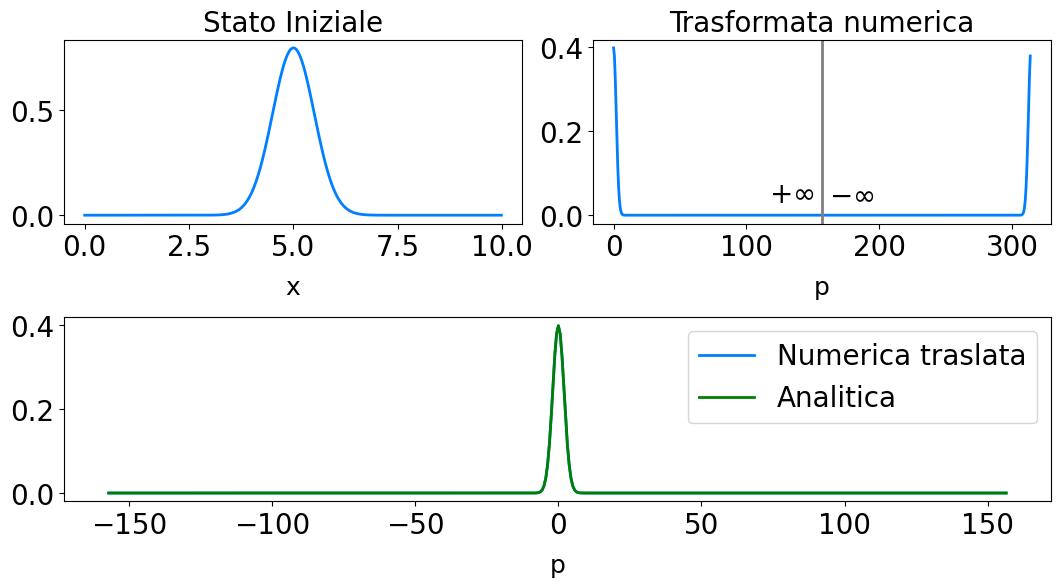
\includegraphics[width = 0.7\textwidth]{immagini/fourier.png}
    \caption{Modulo della trasformata di Fourier di una funzione gaussiana centrata in $x_0 = 5$. Notare come per ottenere la vera rappresentazione fisica nello spazio dei momenti sia necessario eseguire una traslazione rigida della soluzione numerica per $p >   \pi \hbar \, N / L  $}
    \label{fig:dft_shift}
\end{figure}
La discretizzazione dei valori introduce un'altra problematica. La trasformata discreta mappa tutti i valori di $\tilde{\psi}(p)$ in un intervallo che non è simmetrico rispetto all'origine, come fa invece la trasformata continua. Se si considera un periodo $ 0 \le p \le 2 \pi \hbar \, N / L  $ in questo spazio sono mappati tutti i valori di $p$ da $- \infty$ a $+ \infty$, ma sono disposti in ordine inverso. Nella prima metà, tra $ 0 \le p \le \pi \hbar \, N / L  $, sono mappati i valori tra $0$ e $+ \infty$, mentre nella seconda metà tra  $ \pi \hbar \, N / L  < p \le 2 \pi \hbar \, N / L $ sono riportati i valori corrispondenti all'intervallo tra $- \infty$ e $0$. Per costruire, quindi, la vera rappresentazione fisica della funzione d'onda nello spazio dei $p$ è necessario eseguire una traslazione rigida della $\tilde{\psi}(p)$ dall'intervallo $ \pi \hbar N / L < p \le 2 \pi \hbar \, N / L $ all'intervallo $ - \pi \hbar \, N / L  < p \le 0 $, come si può vedere dall'esempio riportato in figura (\ref{fig:dft_shift}).


\section{Conidizioni e vincoli sul sistema} %{Limiti e criticità}
\label{sec:limits}

I principali limiti della simulazione sono dovuti al processo di discretizzazione. 
La discretizzazione dello spazio impone ovvi limiti sulla scelta dei parametri spaziali, poiché essendo lo spazio della simulazione limitato, si perde informazione su qualsiasi oggetto definito al di fuori dell'intervallo $ 0 \le x \le L$. È quindi banale, ma necessario, fare in modo che la funzione d'onda sia interamente definita all'interno dell'intervallo, a meno di porzioni infinitesime. 

La discretizzazione spaziale introduce, inoltre, due criticità dovute alla natura della trasformata discreta di Fourier. In prima istanza bisogna porre particolare attenzione alla scelta dello stato iniziale, poiché non solo è limitato lo spazio diretto, ma lo è anche lo spazio dei momenti. La discretizzazione pone dei limiti non solo sui parametri spaziali della funzione d'onda, ma anche su quei parametri capaci di modificare la forma del profilo nello spazio nei momenti. Nuovamente è necessario che, a meno di infinitesimi, tutta l'informazione nello spazio dei momenti sia contenuta nell'intervallo $ - \pi \hbar \, N / L  < p \le \pi \hbar \, N / L  $. 
Inoltre la periodicità della trasformata di Fourier genera un effetto per cui un per profilo uscente da un estremo dello spazio viene propagata l'evoluzione come entrante dall'altro estremo dello spazio. Tale effetto disturba l'evoluzione della funziona d'onda originale, rendendola scorretta. Scegliendo opportunamente i parametri, è possibile ovviare a questo problema facendo in modo che le conseguenze di questo effetto si manifestino a tempi maggiori di quelli necessari ad ottenere i risultati desiderati. 
\textcolor{red}{ Se, però, si volesse simulare l'andamento di un sistema per tempi lunghi è possibile ovviare a questo problema modificando la forma del potenziale agli estremi dell'intervallo. Se, infatti, si modifica $V$ in maniera tale per cui 
\begin{equation}
    V'(x) = 
        \begin{cases}
            V(x) \quad &\lambda < x < L - \lambda \\ 
             \exp \left(-i \, s\right) &\quad  \text{altrove}
        \end{cases}
    \quad s, \lambda \in \mathbb{R} \, \text{,}
    \label{eq:stp_bound}
\end{equation}
risulterà che la funzione d'onda verrà smorzata esponenzialmente ai bordi. La scelta di $s$ e $\lambda$ deve essere opportunamente valutata in modo da ottenere il risulato desiderato. Per valori di $s$ ed $\lambda$ troppo piccoli lo smorzamento non sarà sufficiente a rendere l'effetto trascurabile. D'altra parte all'aumentare di $s$ aumenta la riflessione dovuta allo smorzamento, altro effetto da voler minimizzare. }

La discretizzazione temporale introduce un valore massimo possibile per il potenziale, dovuto ai termini $ \exp \left(- i V c_{j} \, \delta t\right)$, che sono funzioni periodiche. \textcolor{red}{Dovrei entrare più nel dettaglio?} %più dettagli? Potrei introdurre una parametrizzazione lineare per V e far vdere che per |V| > \frac{2 \pi}{\delta t c_j} rimappo gli stessi valori dell'intervallo 0 \le |V| \le \frac{2 \pi}{\delta t c_j}
Bisogna, quindi, considerare la seguente condizione
\begin{equation}
    \underset{[0, L]}{\max} \; \abs{V(x)} < \frac{2 \pi}{\delta t \, c_{j}} \, \text{.}
    \label{eq:V_max}
\end{equation}
In alcuni casi è possibile ovviare a questa problematica tramite opportune estensioni della funzione d'onda, vedi la sezione \ref{sec:inf}



\chapter{Validazione del codice}
\label{ch:Validazione}

Per collaudare %mettere alla prova
il metodo risolutivo sono stati implementati vari potenziali di cui si conosce la soluzione analitica per poter confrontare i risultati numerici con l'evoluzione esatta. In tutte le simulazioni è stato utilizzato come operatore di evoluzione quello in eq. (\ref{eq:LT_2}), considerato come il miglior compromesso tra precisione e costo computazionale.


\section{Particella libera}
\label{sec:free}

\subsection{Pacchetto d'onde gaussiano}
\label{sec:WP_gaussiano}

Si ricorda la definizione di pacchetto d'onda per le onde piane, poiché è stato scelto come principale stato iniziale all'interno delle simulazioni.
\begin{equation}
    \centering
    \psi(q, 0) = \frac{1}{\sqrt{2 \pi}} \int_{- \infty}^{+ \infty} dk \; g(k) \exp \left(ikq\right) \, \text{,}
    \label{eq:WP}
\end{equation}
dove $g(k)$ rappresenta una distribuzione di probabilità che fissa i contributi per ogni valore di $k$.
Per un pacchetto gaussiano\footnote{Dove $g(k)$ prende la forma di distribuzione gaussiana} e sostituendo le definizioni
\begin{equation}
    \hbar k \equiv p - p_0 \, \text{,}   \quad q \equiv x - x_0 \, \text{,}
    \label{eq:def_kq}
\end{equation}
l'eq. (\ref{eq:WP}) si riduce a 
\begin{equation}
    \centering
    \psi(x, 0) = \left( \frac{2}{ \pi \sigma^2} \right)^{\nicefrac{1}{4}} \exp \left(-i \frac{p_{0}}{\hbar} (x -x_0)\right) \exp \left(-\frac{(x -x_0)^2}{\sigma^{2}}\right) \, \text{,}
    \label{eq:WP_gaus}
\end{equation}
dove $p_0$ rappresenta lo sfasamento del pacchetto nello spazio dei momenti ed è la grandezza che controlla l'energia cinetica associata al pacchetto $T = p_{0}^{2} / 2m$. In figura {\ref{fig:free_p_view}} viene riportato un esempio.

\begin{figure}
    \centering
    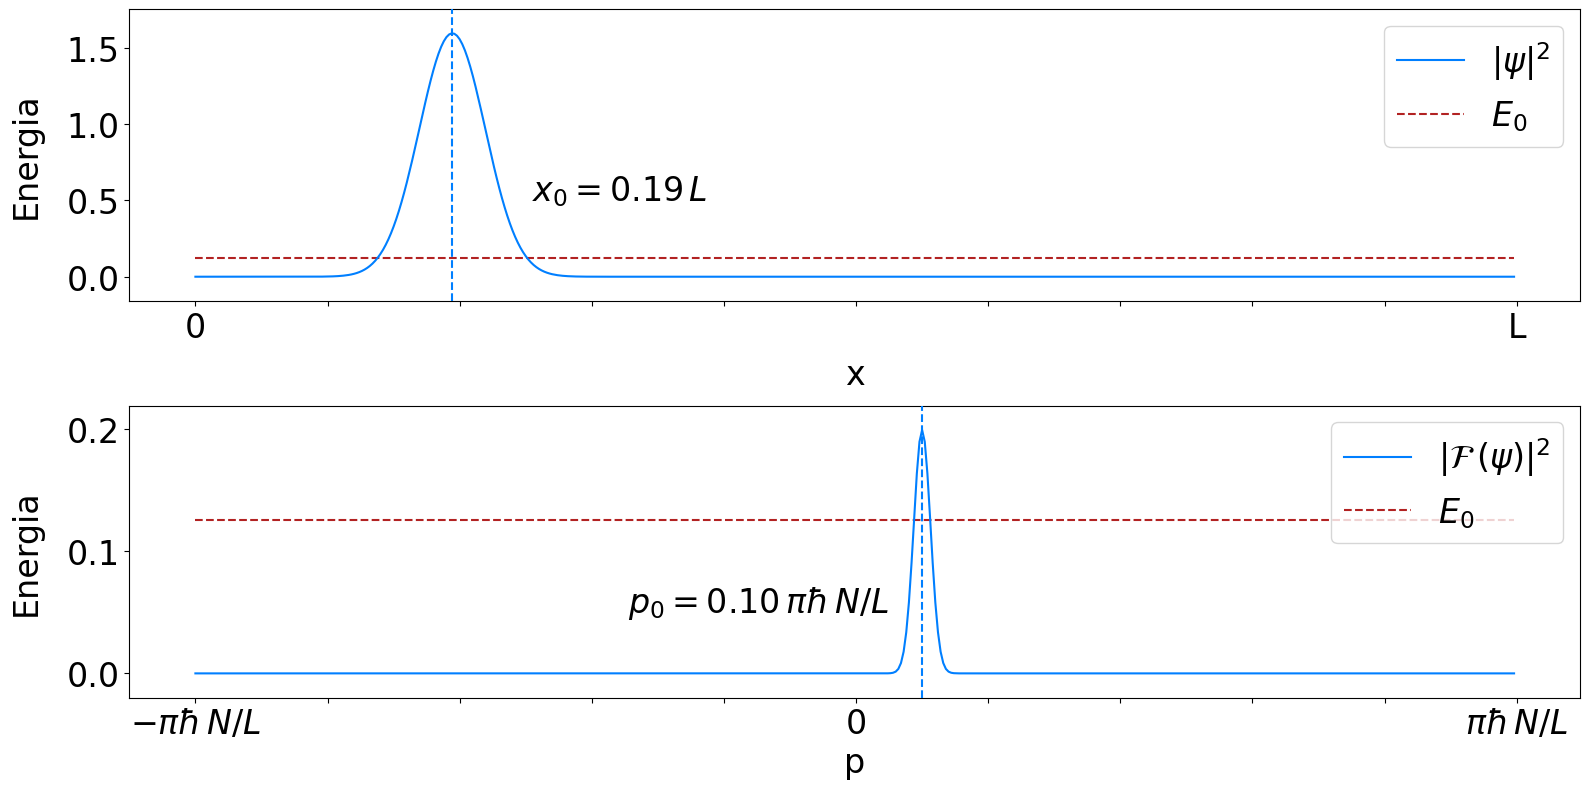
\includegraphics[width = \textwidth]{immagini/free_p_view.png}
    \caption{Rappresentazione dello stato inziale per un pacchetto gaussiano di onde piane, sia nello spazio diretto sia nello spazio dei momenti.}
    \label{fig:free_p_view}
\end{figure}

\subsection{Evoluzione analitica}

Con potenziale di particella libera si intente una configurazione a potenziale costante $V(x) = 0$. In tale configurazione si può considerare la soluzione analitica per l'evoluzione di un pacchetto d'onde del tipo in eq. (\ref{eq:WP_gaus}). 
Data l'eq. (\ref{eq:Sc_1D}), con $V(x) = 0$, questa è risolta per ogni funzione del tipo
\begin{equation}
    \centering
    \psi(x, t) = A \exp \left(i(kx - \omega t)\right) \qquad \text{con}  \quad \omega = \frac{\hbar k^2}{2m} \, \text{.}
    \label{eq:plane_wave}
\end{equation}
Dal principio di sovrapposizione si ottiene che
\begin{equation}
    \centering
    \psi(q,t) = \frac{1}{\sqrt{2 \pi}} \int_{- \infty}^{+ \infty} dk \; g(k) \exp \left(i(kq - \omega t)\right) \, \text{.}
    \label{eq:WP_ev}
\end{equation}
Considerando un pacchetto gaussiano e sostituendo le definizioni in eq. (\ref{eq:def_kq}), si ottiene una funzione analitica per l'evoluzione del pacchetto nel tempo \cite{CT:QM}
\begin{equation}
    \centering
    \psi(x,t) = 
    \left( \frac{2 \sigma^2}{\pi} \right)^{\nicefrac{1}{4}} 
    \left( \sigma^4 + \frac{4 \hbar^2 t^2}{m^2}   \right)^{\nicefrac{-1}{4}}
    \exp \left(i \frac{p_0}{\hbar} x\right) 
    \exp \left( - \frac{\left[ x - p_0 t / m \right]^{2}} {\sigma^2 - 2 i \hbar t / m} \right)
    e^{i \phi} \, \text{,}
    \label{eq:WP_gaus_ev}
\end{equation}
\begin{equation}
    \centering
    \text{con} \quad \phi = - \frac{1}{2} \arctan (\frac{2 \hbar t}{m \sigma_0^2}) - \frac{p_0^2}{2 m \hbar} t  \, \text{.}
\end{equation}
In figura (\ref{fig:free_ev}) si riporta il confronto tra la soluzione numerica e quella analitica per alcuni tempi successivi.

\begin{figure}
    \centering
    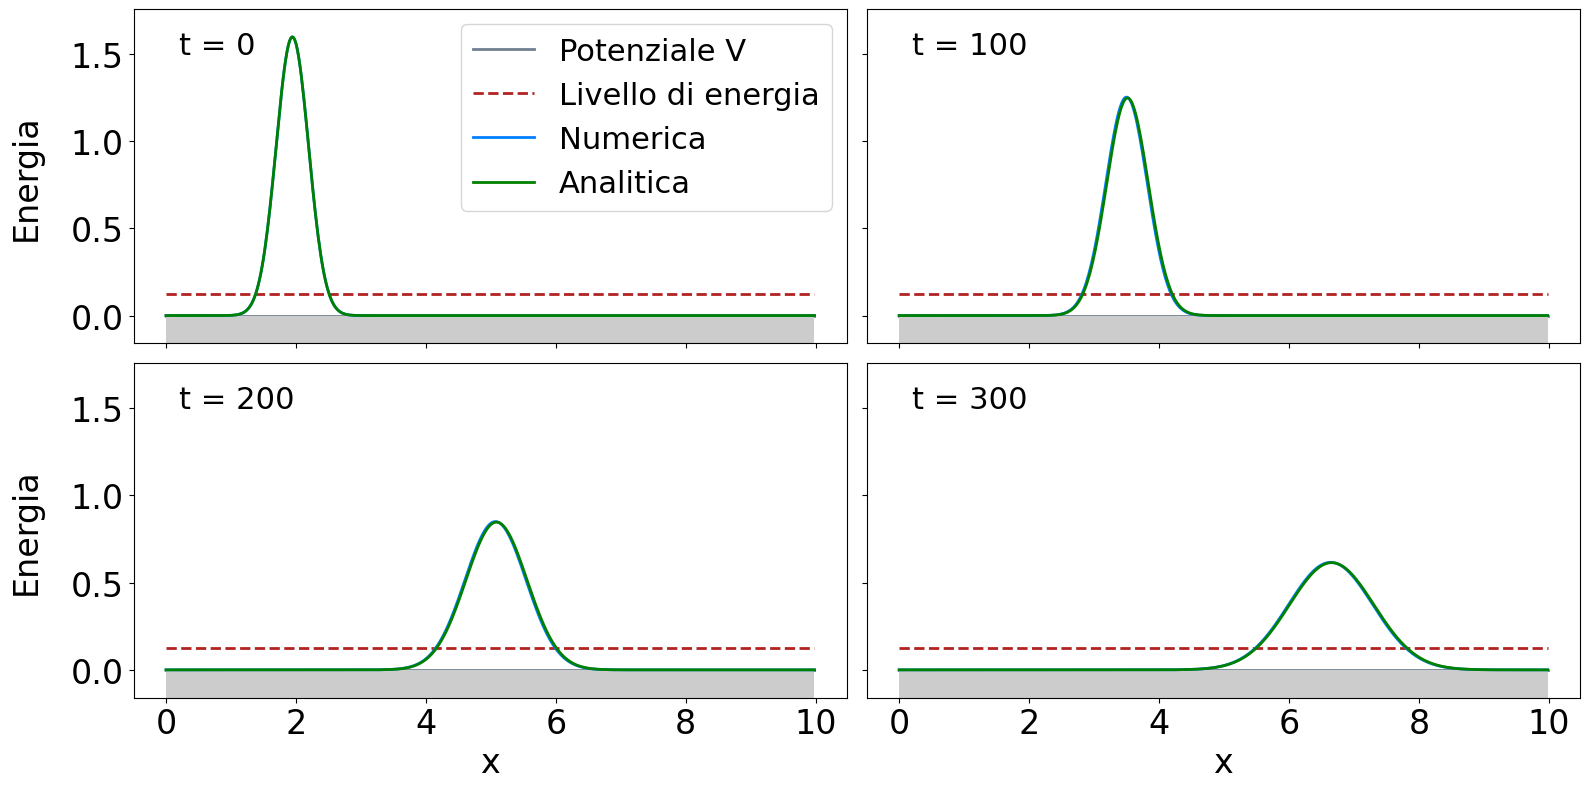
\includegraphics[width = \textwidth]{immagini/free_ev.png}
    \caption{Confronto tra soluzione numerica e soluzione analitca per una particella libera. Si può notare un'ottima sovrappsozione tra le due.}
    \label{fig:free_ev}
\end{figure}


\section{Oscillatore armonico}
\label{sec:arm}

L'oscillatore armonico quantistico è definito da 
\begin{equation}
    \centering
    V(x) = \frac{1}{2} m \omega^2 (x -x_0)^2 \, \text{.}
\end{equation}
Si ricordano i principali risultati ottenuti dalla soluzione dell'equazione di Schr\"odinger stazionaria
\begin{equation}
    \centering
    E_n = (\frac{1}{2} + n) \hbar \omega \, \text{,} \qquad \psi_{n} = \left( \frac{\beta^2}{\pi} \right)^{\nicefrac{1}{4}} \frac{1}{\sqrt{2^{n} \, n!}} \exp \left(-\frac{- \beta^2 x^2}{2}\right) H_{n}(\beta x) \, \text{,}
    \label{eq:arm_res}
\end{equation}
\begin{equation}
    \centering
    \text{con}  \quad \beta = \sqrt{\frac{m \omega}{\hbar}} \, \text{.}
\end{equation}
È noto che se si considera l'eq. (\ref{eq:U}) per gli stati stazionari questa si riduce a 
\begin{equation}
    \centering
    \psi_{n}(x, t) = \exp \left( - \frac{i}{\hbar} E_n t \right) \psi_{n} (x,0)      \, \text{.}
    \label{eq:ev_eigenstate}
\end{equation}
Se inoltre si considera come stato iniziale una combinazione lineare di autostati è possibile trovare l'evoluto temporale combinando le evoluzioni di ogni singolo autostato
\begin{equation}
    \centering
    \psi(x, t) = \sum_{k} c_{k} \, \exp \left( - \frac{i}{\hbar} E_k t \right) \psi_k (x,0) \qquad \text{con} \quad\psi(x,0) = \sum_{k} c_{k} \,  \psi_k (x,0)        \, \text{,}
    \label{eq:ev_combinazione}
\end{equation}
che è una funzione analitica esatta.

\textcolor{red}{ In figura %(\ref{fig:superpos}) 
riportano il confronto tra la soluzione numerica e l'evoluzione analtica per la sovrappoizione di auotostati dell'oscillatore armonico
\begin{equation}
    \centering
    \psi(x, 0) = \frac{1}{\sqrt{2}} \left( \ket{0} + \ket{1} \right)   \, \text{.}
    \label{eq:superpos}
\end{equation} 
}

\section{Stati coerenti}
\label{sec:coherent}

Con stati coerenti \cite{CT:QM} si intendono gli autostati dell'operatore di distruzione dell'oscillatore armonico. Sono divenuti celebri, poiché vennero utilizzati da Schr\"odinger come dimostrazione del principio di corrispondenza. Tali stati, infatti, sono caratterizzati da una dinamica molto simile al comportamento oscillatorio di un oscillatore armonico classico. 

Non esiste una definizione analitica per gli stati coerenti, poiché sono definiti tramite una sovrapposizione infinita, del tipo in eq. (\ref{eq:ev_combinazione}), di autostati di oscillatore armonico nel seguente modo
\begin{equation}
    \centering
    \ket{\alpha} = \exp \left(- \frac{|\alpha|^2}{2}\right) \sum_{n=0}^{+ \infty} \left( \frac{\alpha^n}{n!} \right) \ket{n} \, \text{.}
    \label{eq:def_coherent}
\end{equation} 
Numericamente non è possibile estendere la somma a $+\infty$, per questo è necessario troncarla ad un valore finito, all'interno del codice è stato fissato a 170.

L'evoluzione analitica per il modulo quadro di uno stato coerente corrisponde ad una traslazione rigida di una gaussiana con 
\begin{equation}
    \centering
    \expval{x}_{t} = A \, cos(\theta - \omega t) \, \text{,} \quad
    \expval{p}_{t} = m \omega A \, sen(\theta - \omega t) \qquad
    \text{dove} \quad A = \sqrt{\frac{2 \hbar}{m \omega}} |\alpha| \, \text{,}
    \label{eq:coherent_an}
\end{equation}
che corrispondono alle soluzioni classiche dell'oscillatore armonico.

In figura (\ref{fig:coherent_ev}) è riportato il confronto tra la soluzione analitica e numerica per l'evoluzione di uno stato coerente, mentre in sezione (\ref{sec:Wp_arm}) si studia l'evoluzione di pacchetto gaussiano di onde piane anche in confronto ad uno stato coerente.

\begin{figure}
    \centering
    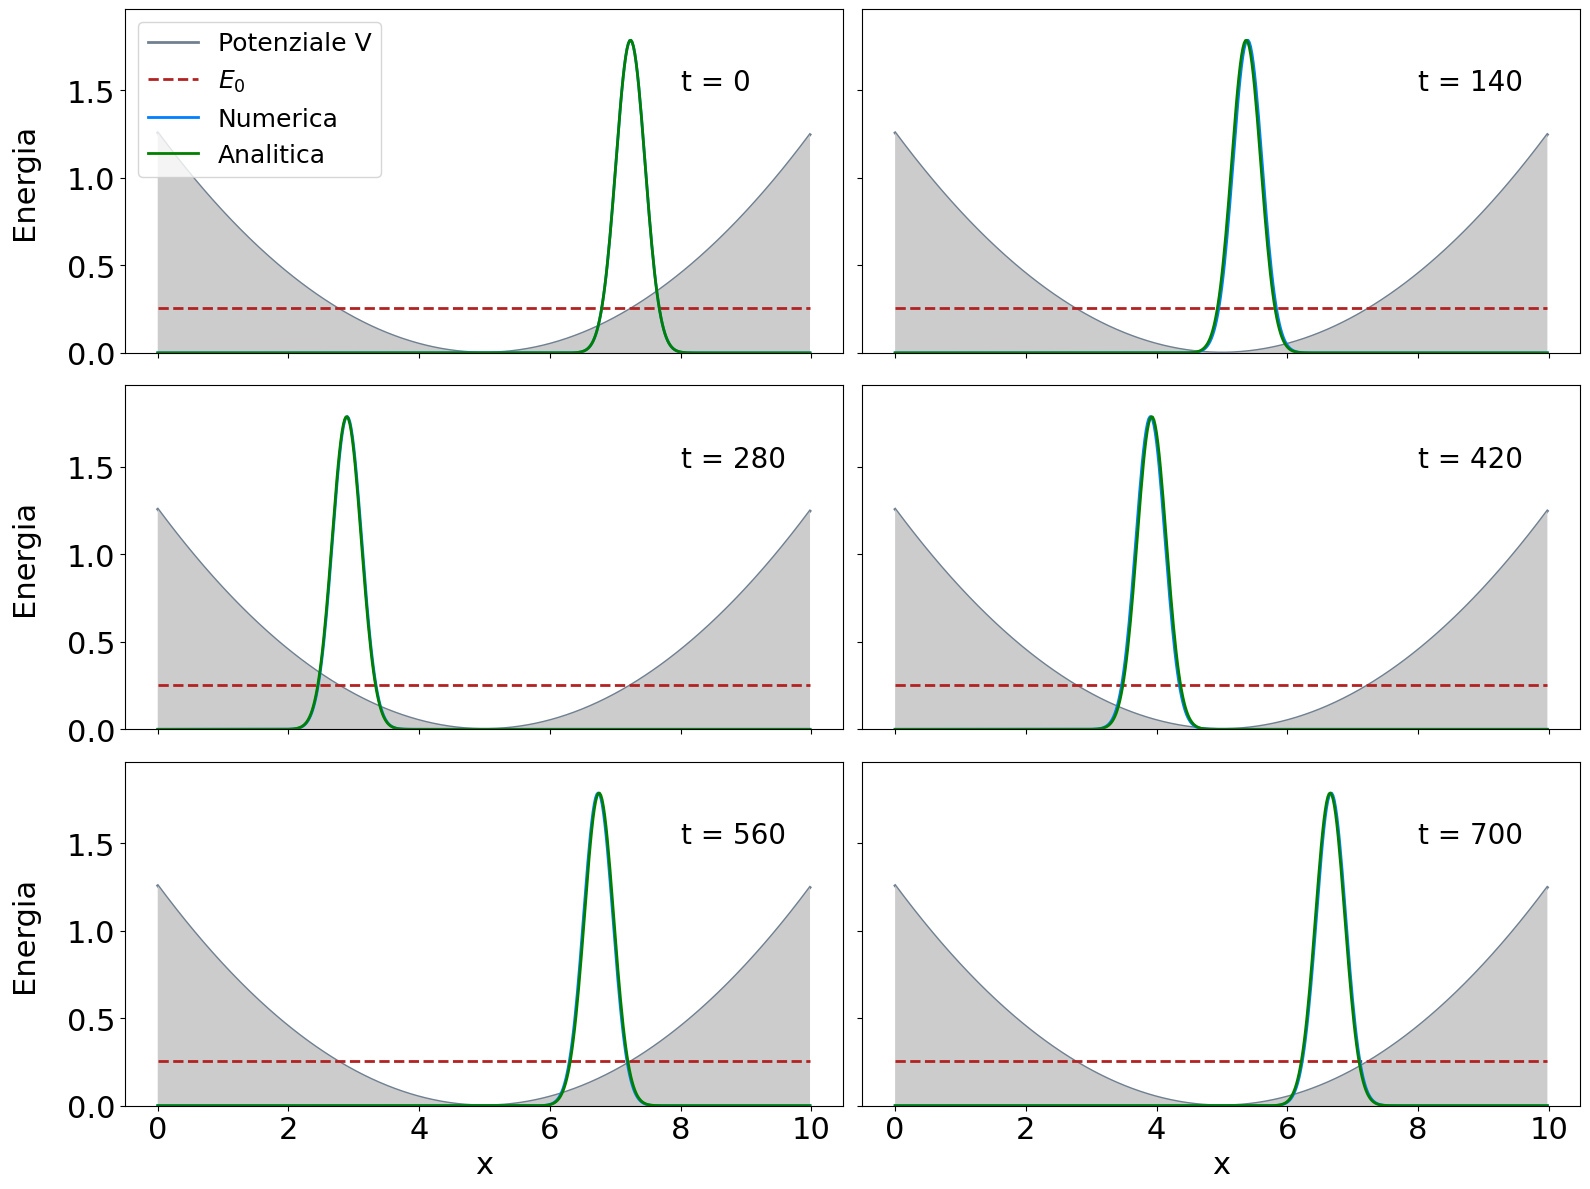
\includegraphics[width = \textwidth]{immagini/coherent_ev.png}
    \caption{Confronto tra soluzione numerica e soluzione analitica per uno stato coerente. Si noti come le dimensioni del pacchetto di forma gaussiana non vengano deformate durante l'evoluzione.}
    \label{fig:coherent_ev}
\end{figure}



\section{Potenziale di P\"oschl-Teller}
\label{sec:RL}

Il potenziale di P\"oschl-Teller (PT), applicato nel contesto della meccanica quantistica, prende la forma 
\begin{equation}
    \centering
    V(x) = -\frac{\hbar^2 \alpha^2}{2m} \frac{\nu (\nu + 1)}{\cosh^2 \alpha x} \quad \text{.}
    \label{eq:pot_PT}
\end{equation}
Questo potenziale è di particolare importanza poiché si può dimostare che $\forall \nu$ il coefficiente di trasmissione, $T$, per una funzione d'onda incidente sul potenziale risulta essere pari a $1$. Per questo gli viene attribuito l'aggettivo \textsl{reflectionless}.   
Come per il potenziale armonico è possibile risolvere l'equazione agli autovalori per PT con un metodo algebrico, definendo gli operatori di innalzamento e abbassamento, quindi risolvere analiticamente il problema per una qualsiasi combinazione di autostati in analogia con quanto fatto in precedenza. \cite{Jaffe:RL_sol}

Fissando  $\nu = 1$ si ottengono gli autostati e autovalori
\begin{equation}
    \centering
    \psi_{k}(x) = \left[ \frac{i k - \alpha \tanh (\alpha x)}{ik + a}\right] \exp(ikx)  \; \text{,} \quad E_k = \frac{\hbar^2 k^2}{2 m } \quad \text{con} \; k \in \mathbb{R} \, \text{,}
\end{equation}
che generano uno spettro continuo e infinito. Si può, dunque, costruire un pacchetto d'onde di autostati 
\begin{equation}
    \centering
    \psi(x, t) = \frac{1}{\sqrt{2 \pi}} \int_{-\infty}^{+\infty} dk \, A(k) \, \psi_{k}(x) \exp \left(- \frac{i}{\hbar} E_k t \right) \, \text{,}
    \label{eq:WP_RL_def}
\end{equation}
si ricorda che $p - p_0 \equiv \hbar k$.
Fissando $A(k) = (ik + \alpha) \phi_0(k)$, dove $\phi_0(k)$ è la trasformata di Fourier dell'eq. (\ref{eq:WP_gaus}) e risolvendo l'integrale si ottiene la soluzione per l'evoluzione di un pacchetto d'onde gaussiano di autostati di PT
\begin{equation}
    \centering
    \psi(x, t) = N \left[i \frac{p_0}{\hbar} - \frac{x - x_0 - v_{g}t}{ \sigma_0 s_t} - \alpha \tanh (\alpha x) \right] \psi_{G}(x,t)    \, \text{,}
    \label{eq:WP_RL_ev}
\end{equation}
\begin{equation}
\text{con} \quad s_t = \frac{\sigma_0}{2} \left(1 + i \frac{2 \hbar t}{ m \sigma_0^2} \right)
\end{equation}
e dove $\psi_{G}(x,t)$ si riferisce all'evoluzione libera di un pacchetto gaussiano di onde piane, $v_g = p_0 / m$ è la velocità di gruppo.\cite{Mousavi:PL_WP}

In figura (\ref{fig:WP_RL}) si riporta il confronto tra la soluzione numerica e la soluzione analitica, riscontrando una quasi perfertta sovrapposizione.

\begin{figure}
    \centering
    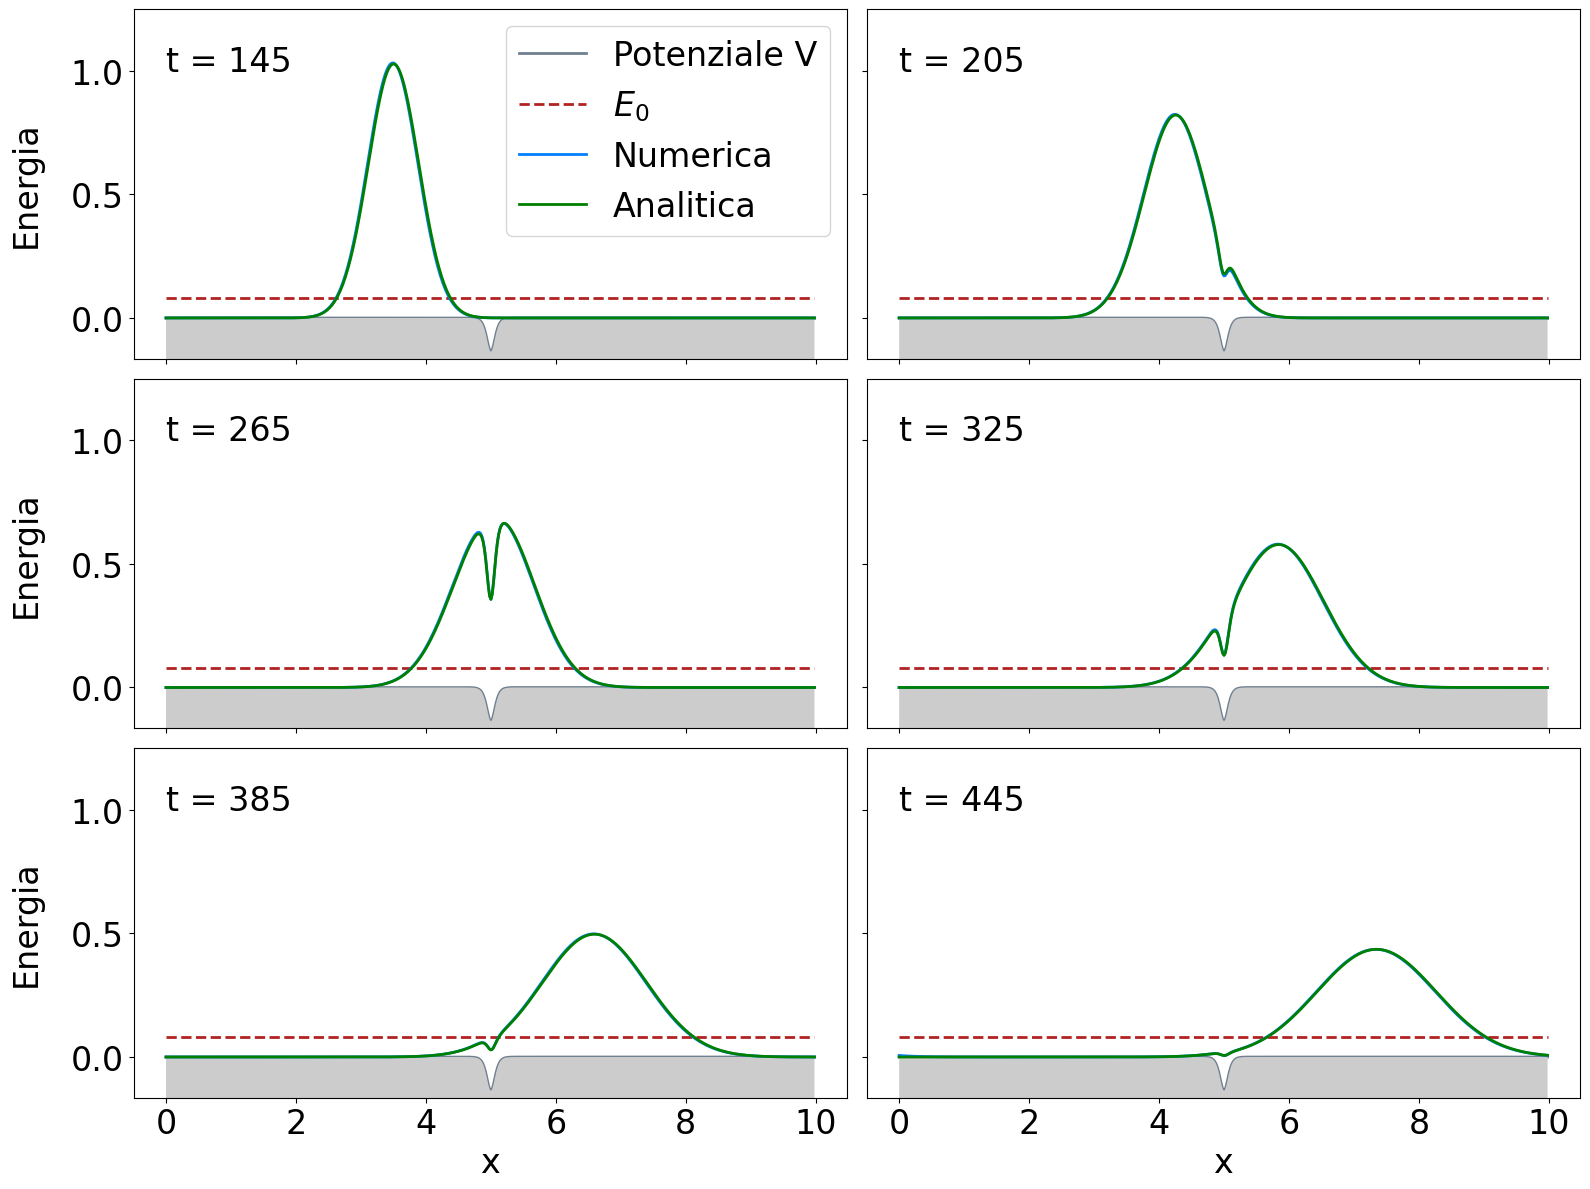
\includegraphics[width = \textwidth]{immagini/WP_RL.png}
    \caption{Confronto tra soluzione numerica e soluzione analitica per un pacchetto gaussiano di autostati di PL. Ancora una volta si ottiene un ottimo accordo tra la simulazione numerica e l'evoluzione esatta.}
    \label{fig:WP_RL}
\end{figure}


\chapter{Applicazioni}
\label{ch:applicazioni}

L'utente tramite l'interfaccia ha la possibilità di scegliere tra alcuni potenziali pre-impostati:
\begin{itemize}[nolistsep]
    \item particella libera,
    \item oscillatore armonico,
    \item buca e barriera finita di potenziale,
    \item gradino di potenziale,
    \item barriera coulombiana semplificata ,
    \item potenziale \textsl{reflectionless} di P\"oschl-Teller,
    \item barriera infinita.
\end{itemize}
Da combinare con i seguenti stati iniziali:
\begin{itemize}[nolistsep]
    \item pacchetto gaussiano di onde piane, 
    \item autostati dell'oscillatore armonico e loro sovrapposizioni,
    \item stati coerenti,
    \item pacchetto gaussiano di autotati del potenziale di PL.
\end{itemize}
In questa sezione non solo si riportano alcuni dei risultati ottenuti partendo dagli stati sopracitati, ma anche altre soluzioni di particolare interesse.


\section{Buca finita di potenziale}
\label{sec:finite_hole}

La buca finita è definita tramite
\begin{equation}
    \centering
    V(x) =
    \begin{cases}
        \; -V_0  \quad &\text{per} \quad a \le x \le b \\
        \; 0 \qquad &\text{altrove}      \; \text{.}
    \end{cases}
\end{equation}
La soluzione di questo problema permette di mettere in evidenza un fenomeno caratteristico della meccanica quantistica: la riflessione di una particella può avvenire anche in corrispondenza di un caduta di potenziale. 
%ben riassunto nella frase di David Jeffrey Griffiths: \textcolor{red}{\dots \dots \dots}
Un tale comportamento è una totale novità rispetto alla meccanica classica. Secondo le equazioni di Newton $m \ddot{\vec{x}} = -\nabla U(\vec{x}, t)$, per cui risulta che in corrispondenza di una differenza di potenziale negativa la particella subisca con certezza una determinata accelerazione nella direzione del moto. In meccanica quantistica questo non è certo che accada, come mostrato in figura (\ref{fig:finite_hole}), infatti esiste una probabilità diversa zero che la particella si trovi nella zona precedente la buca con momento opposto.

\begin{figure}
    \centering
    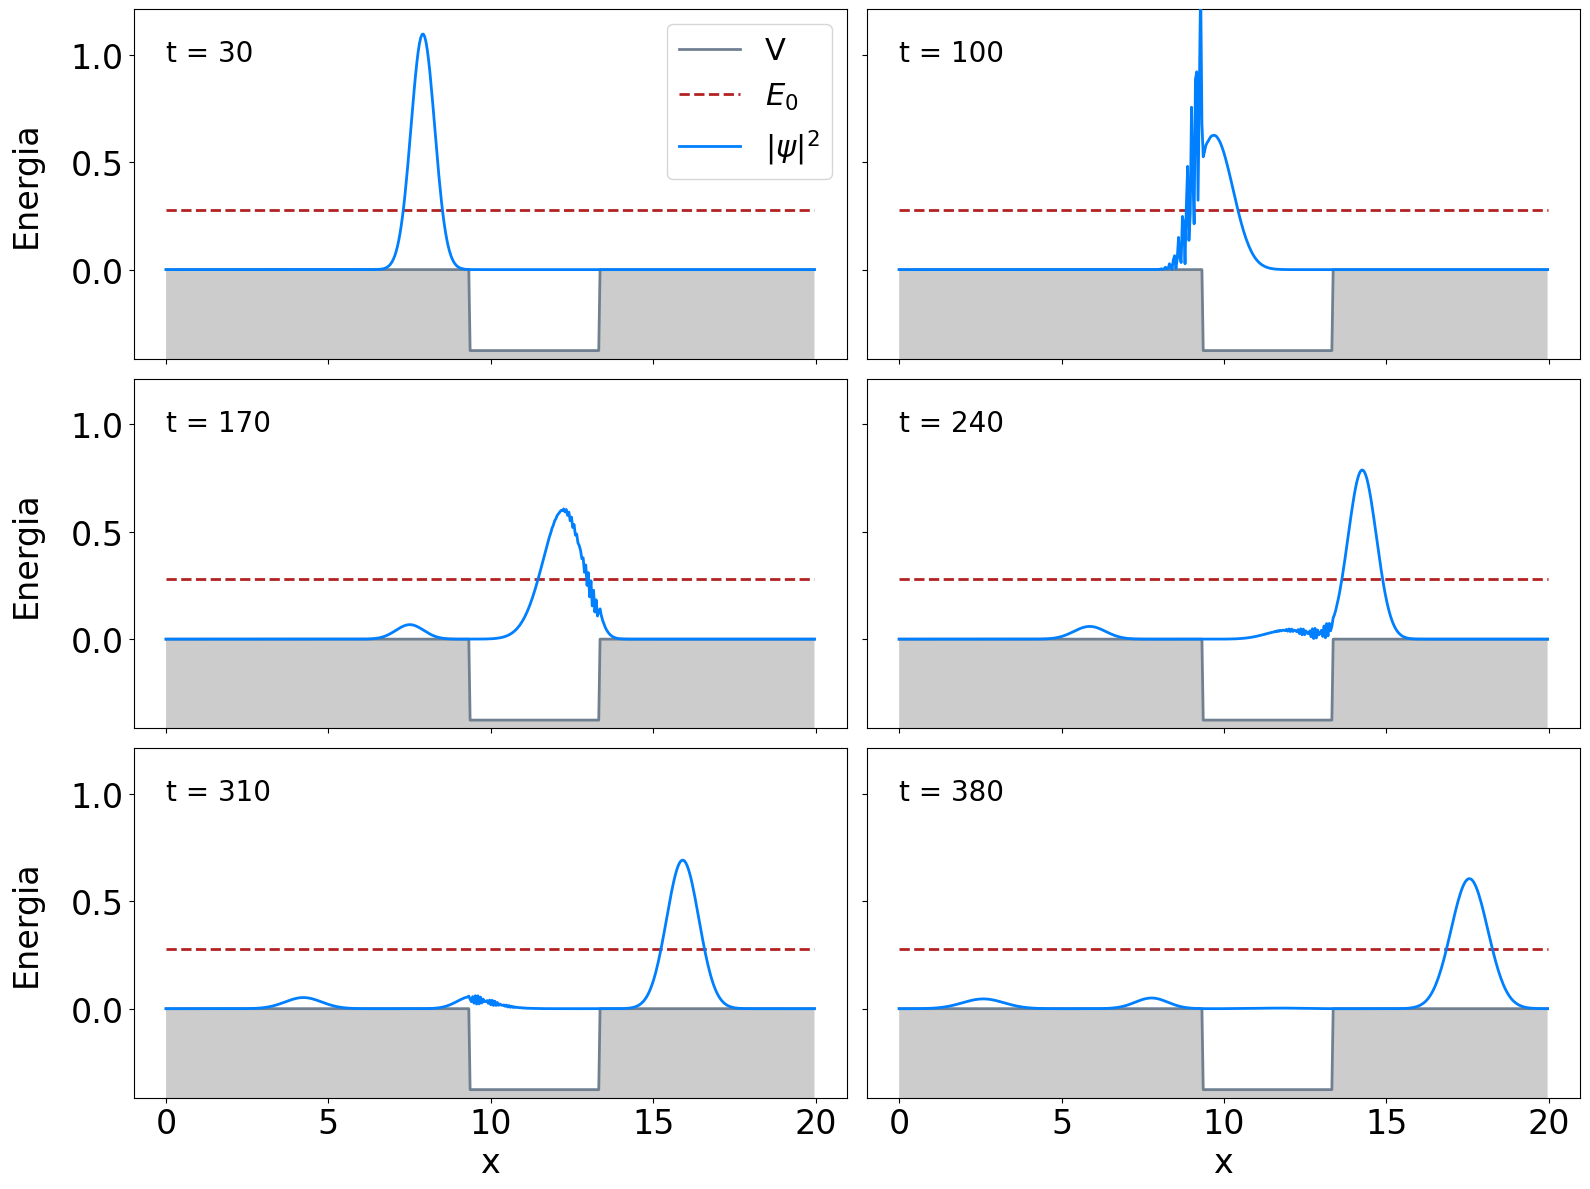
\includegraphics[width = \textwidth]{immagini/hole.png}
    \caption{Evoluzione di un pacchetto gaussiano di onde piano che interagisce con una buca finita di potenziale, si noti il fatto che parte dell'onda viene riflessa, cosa non prevista in meccanica classica.}
    \label{fig:finite_hole}
\end{figure}

\section{Barriera coulombiana semplificata}
\label{sec:coulomb}

È noto come, in prima approssimazione, il potenziale caratteristico per le particelle contenute nel nucleo abbia una forma del tipo
\begin{equation}
    \centering
    V(r) = 
    \begin{cases}
        \, - V_{N} \quad &\text{per} \quad r \le \tilde{R} \\
        \, (Z \, e_0^2) \ (4 \pi \, \epsilon_0) \;\; r^{-1} \quad &\text{per} \quad r > \tilde{R}      \; \text{.}
    \end{cases}
    \label{eq:C_pot}
\end{equation} 
Nel codice è stato implementato un potenziale con lo stesso andamento 
\begin{equation}
    \centering
    V(x) = 
    \begin{cases}
        \, 0 \quad &\text{per} \quad x \le \tilde{x} \\
        \, \left( x - \tilde{x} - (1 / V_0)\right)^{-1} \quad &\text{per} \quad x > \tilde{x}  \; \text{,}
    \end{cases}
    \label{eq:tunnel}
\end{equation} 
per mettere in evidenza un altro fenomeno caratteristico della meccanica quantistica: l'effetto tunnel.
Fenomeno attraverso il quale si giustifica l'espulsione di particelle dal nucleo durante i decadimenti-$\alpha$.
In figura (\ref{fig:tunnel}) si può vedere che nonostante la particella non abbia l'energia sufficiente ad oltrepassare la barriera, \textcolor{red}{secondo la meccanica classica}, una parte della funzione d'onda viene trasmessa.

\begin{figure}
    \centering
    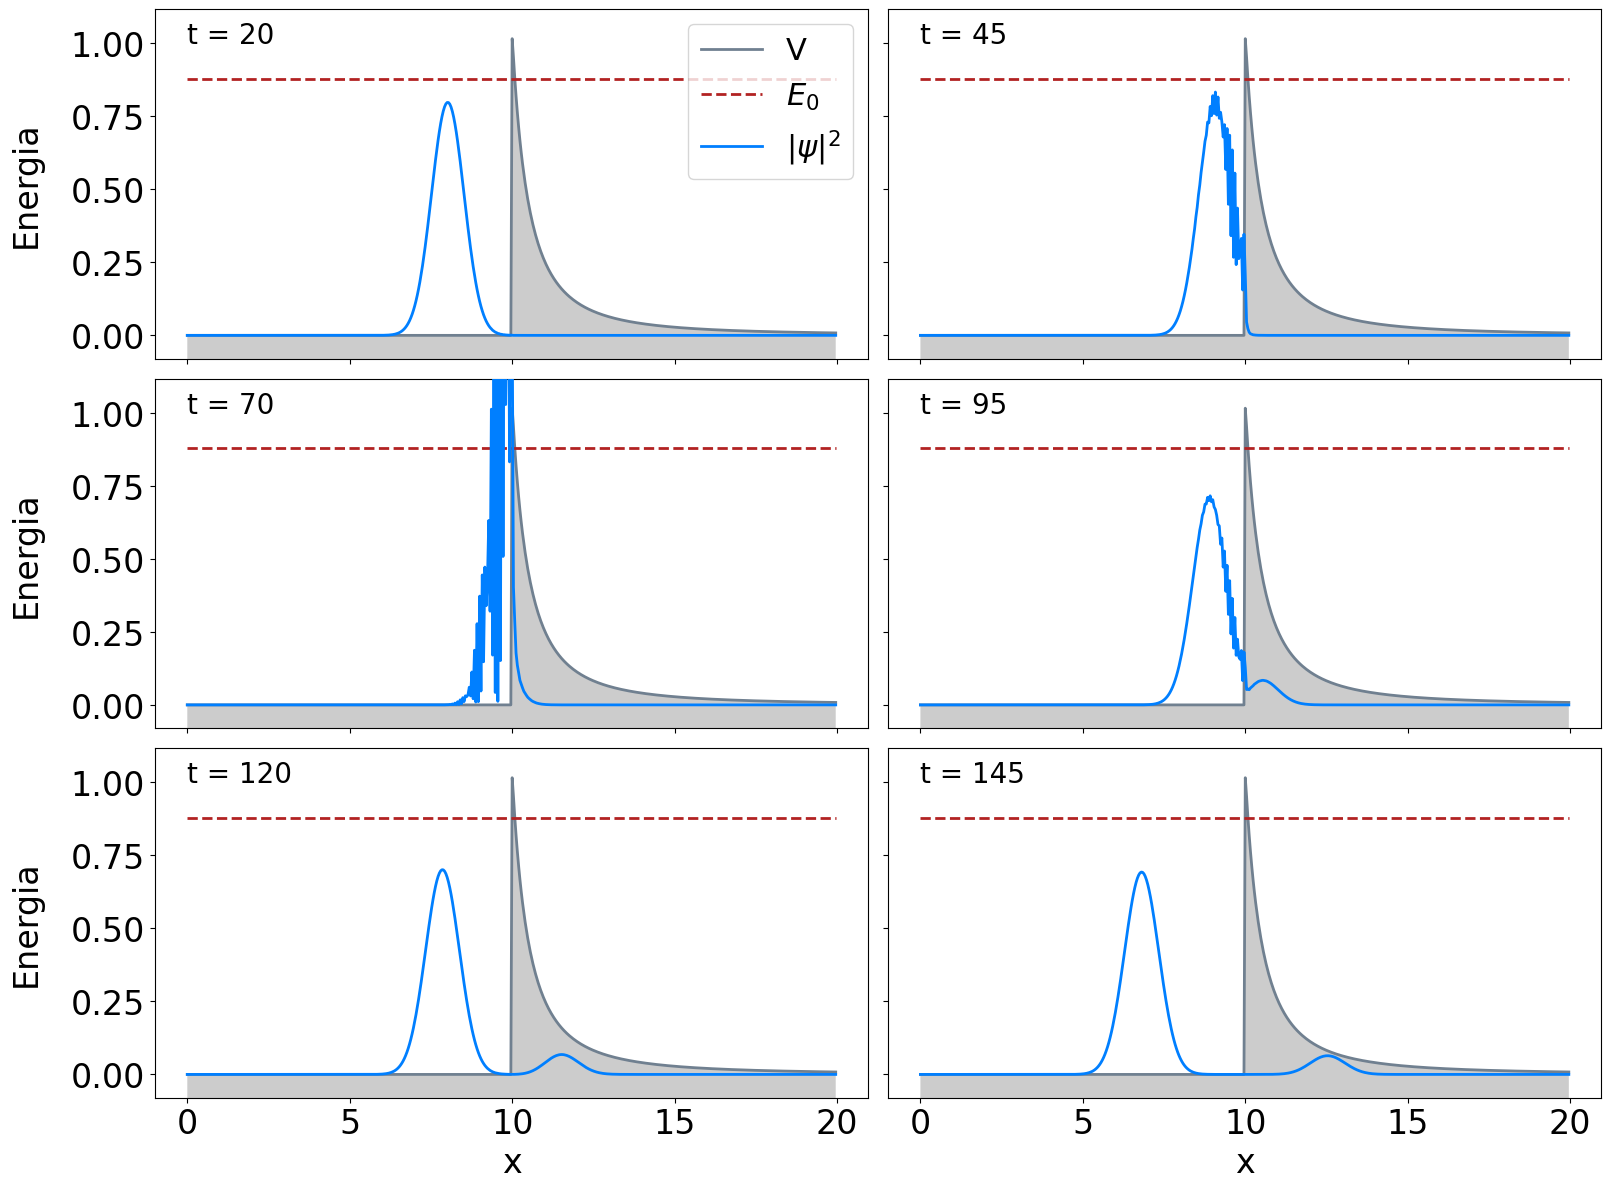
\includegraphics[width = \textwidth]{immagini/tunnel.png}
    \caption{Visualizzazione grafica dell'effetto tunnel per un potenziale Coulombiano.}
    \label{fig:tunnel}
\end{figure}


\section{Pacchetto gaussiano di onde piane in oscillatore armonico}
\label{sec:Wp_arm}

Si ricorda che il comportamento classico di un particella soggetta ad un potenziale armonico è del tutto simile al comportamento di uno stato coerente, come già valutato in sezione (\ref{sec:coherent}).
In questa sezione si vogliono evidenziare le differenze tra uno stato coerente e l'evoluzione di un pacchetto gaussiano di onde piane a cui è associata la stessa energia.
Come si può vedere in figura (\ref{fig:co_vs_WP}), la dinamica del centro di massa del pacchetto di onde piane è facilmente interpretabile tramite la meccanica classica. Infatti il valor medio $\expval{x}$ del pacchetto si sovrappone al valore medio dello stato coerente. D'altra parte mentre gli stati coerenti mantegono le dimensioni del profilo gaussiano, il pacchetto di onde piane subisce continue defomazioni lungo il moto. Emerge un comportamento puramente quantistico per cui la varianza del pacchetto subisce delle contrazioni e delle dilatazioni periodiche di periodo pari alla metà di quello dell'oscillatore armonico classico. \cite{Tsuru:gaus_harmonic}   

\begin{figure}
    \centering
    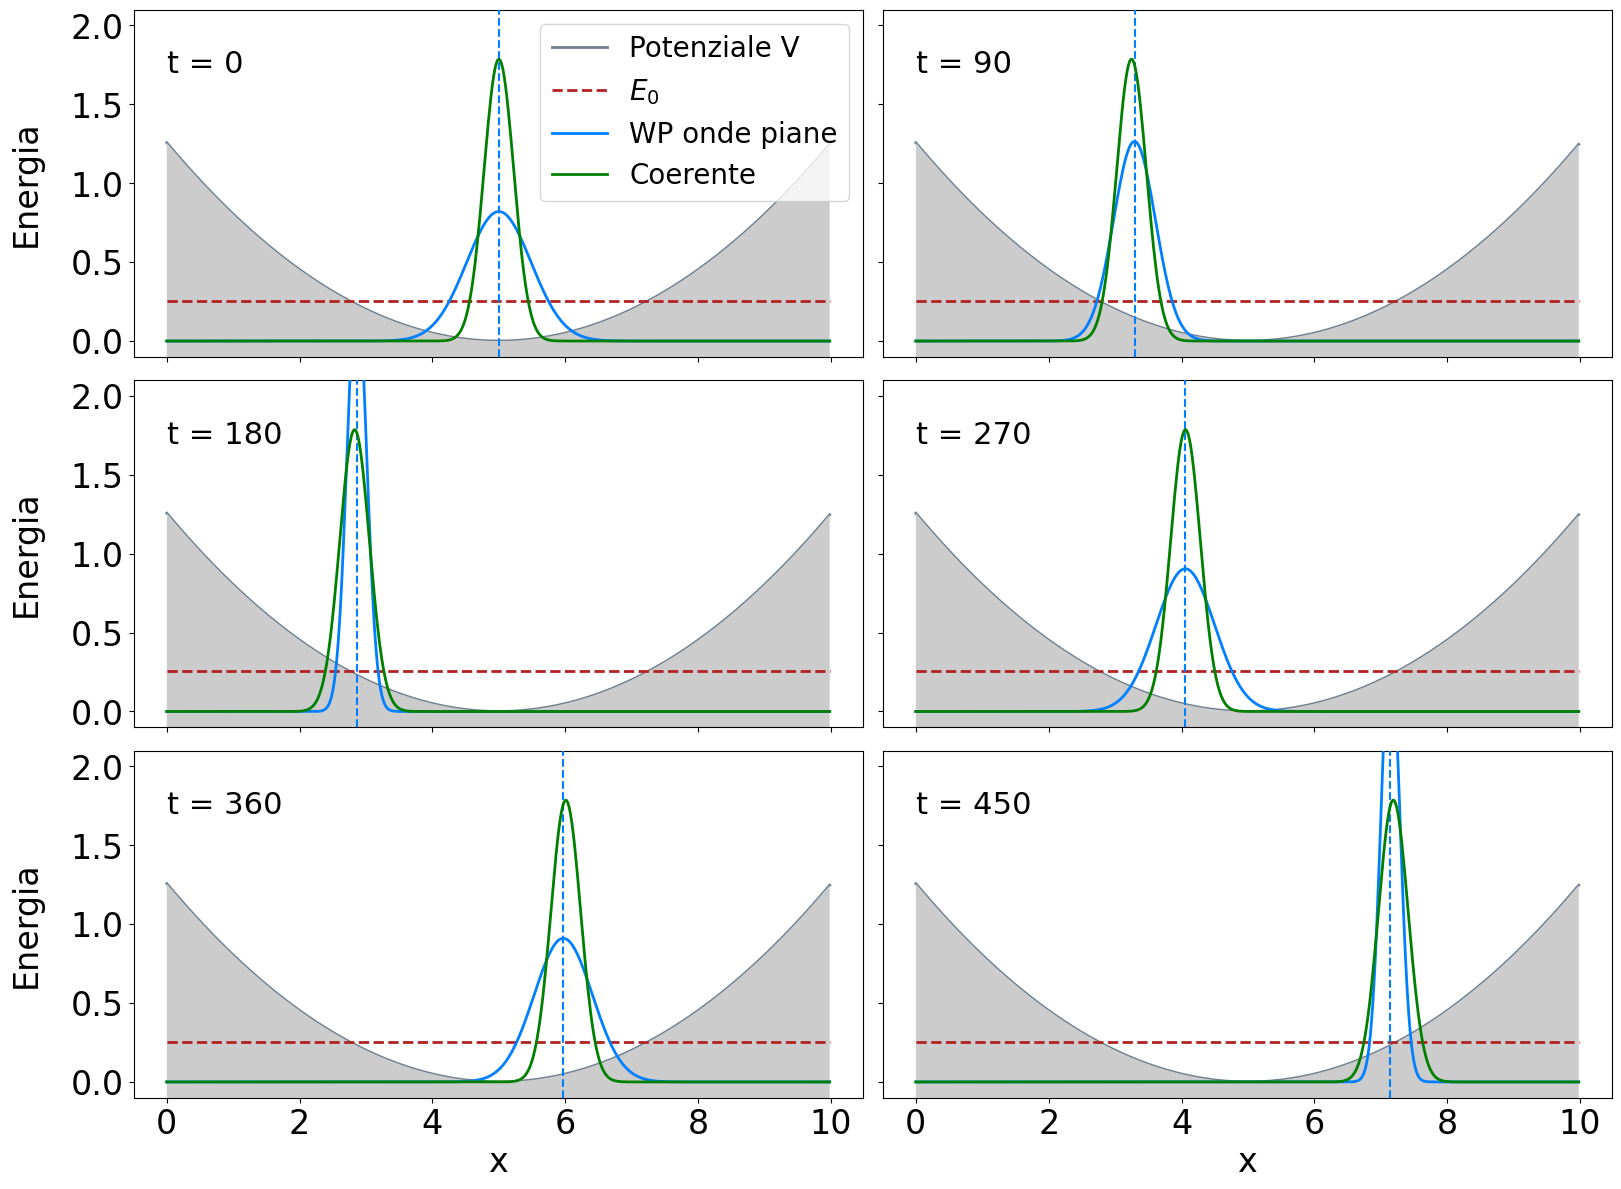
\includegraphics[width = \textwidth]{immagini/coherent_vs_WP.png}
    \caption{Confronto tra l'evoluzione di uno stato coerente e un pacchetto gaussiano di onde piane.}
    \label{fig:co_vs_WP}
\end{figure}

\section{Pacchetto gaussiano di onde piane in potenziale di P\"oschl-Teller}
\label{sec:Wp_PL}

Se si considera un pacchetto gaussiano di onde piane che attraversa un potenziale di P\"oschl-Teller, risulterà che questo verrà interamente trasmesso, come sottolineato in sezione (\ref{sec:RL}).
Si può studiare la deformazione subita dal pacchetto durante il moto e confrontarla con un pacchetto di autostati di PL e l'evoluzione libera.
Come si può riscontrare in figura (\ref{fig:PL_conf}), il pacchetto viene deformato in maniera simile al pacchetto di autosati, subisce un'accelerazione e si ottiene un pacchetto contratto rispetto all'evoluzione libera. Le linee verticali in figura (\ref{fig:PL_conf}) rappresentano il valore medio $\expval{x}$ della corrispettiva funzione d'onda: risulta che il pacchetto d'onde di autostati possiede una velocità di gruppo più alta rispetto al pacchetto gaussiano e risente maggiormente degli effetti del potenziale, è infatti accelerato più velocemente.\cite{Mousavi:PL_WP}

Si è inoltre confrontata l'evoluzione libera di un pacchetto gaussiano di onde piane con la sua evoluzione nel potenziale PL. Risulta che il pacchetto d'onde subisca una deformazione che lo trasla più velocemente rispetto alla propagazione libera lasciandolo più contratto.\cite{Lecker:RL}
\textcolor{red}{ Se si immagina di implementare un reticolo ben dimensionato si potrebbe costruire una macchina che trasporta le particelle da un lato all'altro in maniera molto più efficiente, vedi figura \dots.} 

\begin{figure}
    \centering
    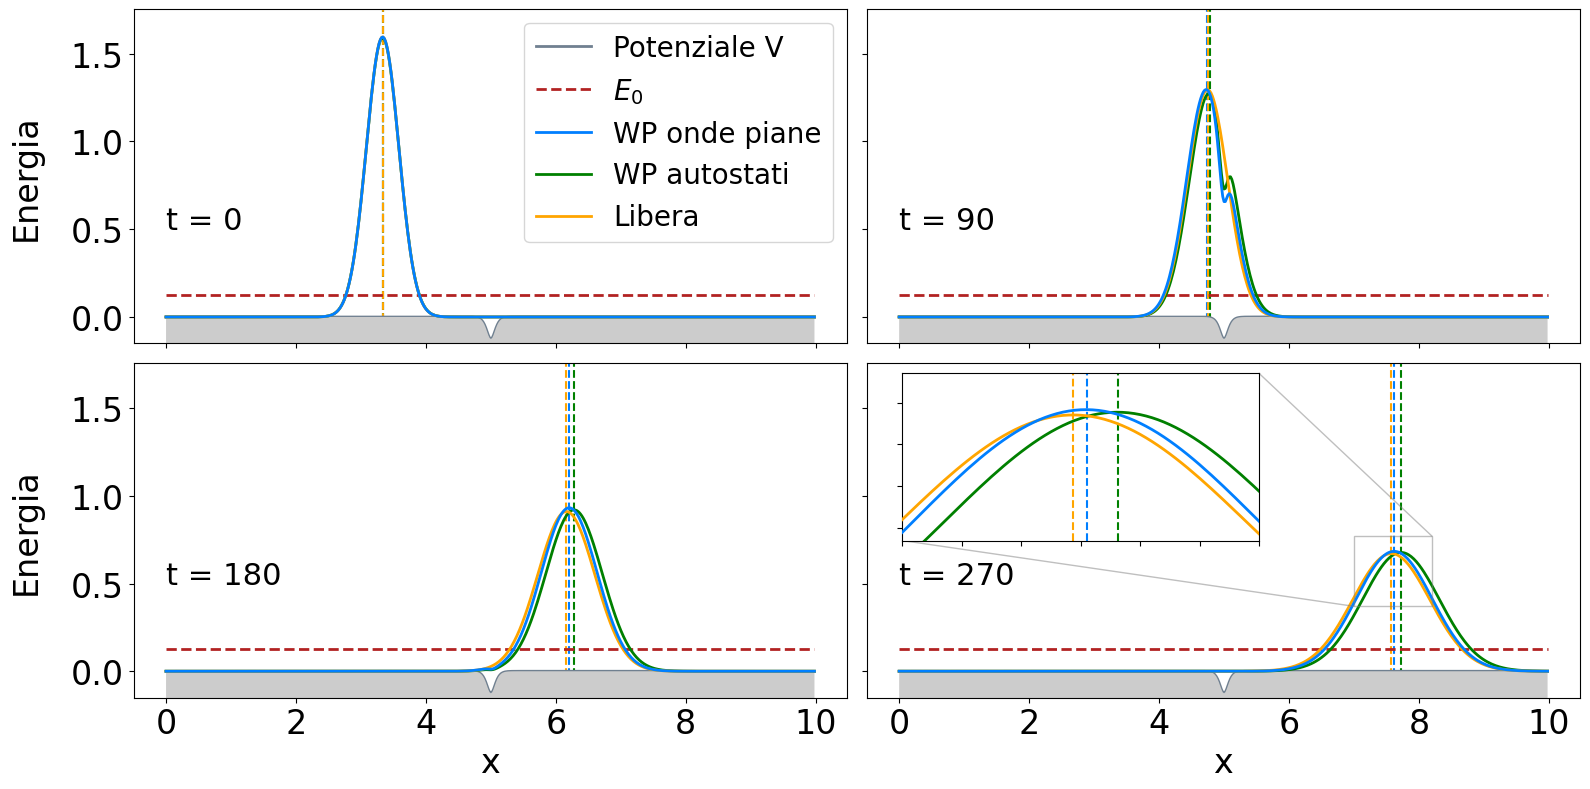
\includegraphics[width = \textwidth]{immagini/PL_num.png}
    \caption{Confronto tra l'evoluzione di uno stato coerente e un pacchetto gaussiano di onde piane.}
    \label{fig:PL_conf}
\end{figure}

\begin{figure}
    \centering
    \includegraphics[width = \textwidth]{immagini/PL_num_zoom.png}
    \caption{Confronto tra l'evoluzione di uno stato coerente e un pacchetto gaussiano di onde piane.}
    \label{fig:PL_conf_zoom}
\end{figure}

\section{Barriera infinita}
\label{sec:inf}

Come riportato in sezione \ref{sec:limits}, non è possibile definire potenziali che non rispettino l'eq. (\ref{eq:V_max}). Il caso particolare della barriera infinita 
\begin{equation}
    V(x) = 
    \begin{cases}
        0 \quad &\text{per} \quad x < x_v \\
        \infty \quad &\text{per} \quad x \geq x_v \; \text{,}
    \end{cases}
    \label{eq:pot_inf}
\end{equation}
è però risolvibile lasciando evolvere un pacchetto opportunamente costruito in un potenziale costante $V = 0$. La presenza di una barriera infinita si traduce matematicamente nell'affermare che 
\begin{equation}
    \psi(x_v, t) = 0 \quad \forall t \; \text{,}
    \label{eq:cond_dir}
\end{equation}
nota anche come condizione al bordo di Dirichlet. 
Se si considera la funzione d'onda antisimmetrica rispetto a $x_v$ di $\psi(x,t)$, costruita con
\begin{equation}
    \psi_{\text{ANT}}(x -x_v, t) =  - \psi(x_v - x , t) \; \text{,} 
\end{equation}    
questa, in un potenziale libero, evolverà in direzione opposta rispetto a $\psi$. Nel momento in cui si considera la sovrapposizione dei due, $\Psi(x,t) = \psi(x, t) + \psi_{\text{ANT}}(x, t)$, si ottiene per costruzione che l'eq. (\ref{eq:cond_dir}) è identicamente verificata $\forall t$. 
La soluzione del problema proposto risulta essere $\Psi(x,t)$ valutata nel'intervallo $(-\infty, 0]$. In figura (\ref{fig:inf}) si riportano i risultati di una simulazione numerica per un pacchetto gaussiano in un potenziale di eq. (\ref{eq:pot_inf}), risolto con il metodo appena descritto.

\begin{figure}
    \centering
    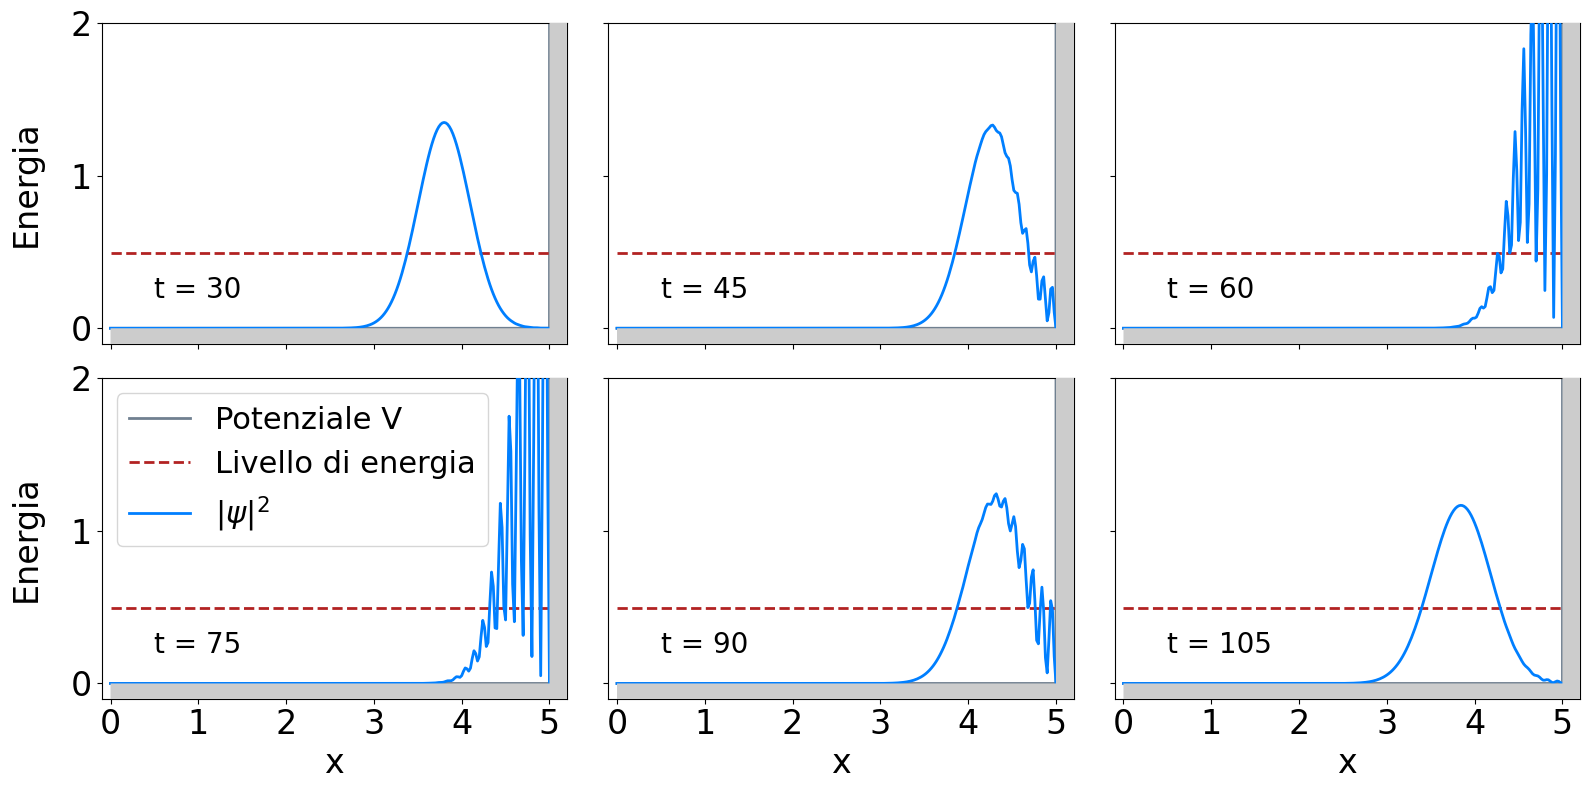
\includegraphics[width = \textwidth]{immagini/inf.png}
    \caption{Evoluzione di un pacchetto gaussiano di onde piano che interagisce con una barriera di potenziale infinita. \textcolor{red}{Se può essere interessante posso sovrappore questa soluzione con la soluzione di un potenziale step con $V_0 \approx V_{MAX}$}}
    \label{fig:inf}
\end{figure}

\section{Potenziale dipendente dal tempo}
\label{sec:t_dep}

Come anticipato è possibile risolvere anche problemi con potenziale dipendente dal tempo.
Come esempio si è scelto di implemenatare un potenziale 
\begin{equation}
   \centering
   V(x) = \alpha \, (x-x_0)^2 +  \frac{| \sin (\omega_v  \, t) |} {1 + \beta \, (x-x_0)^2} \, \text{.}
\end{equation}
Come si può vedere in figura (\ref{fig:t-dep}) è evidente come la funzione d'onda reagisca al potenziale mentre questo cambia forma.

\begin{figure}
   \centering
    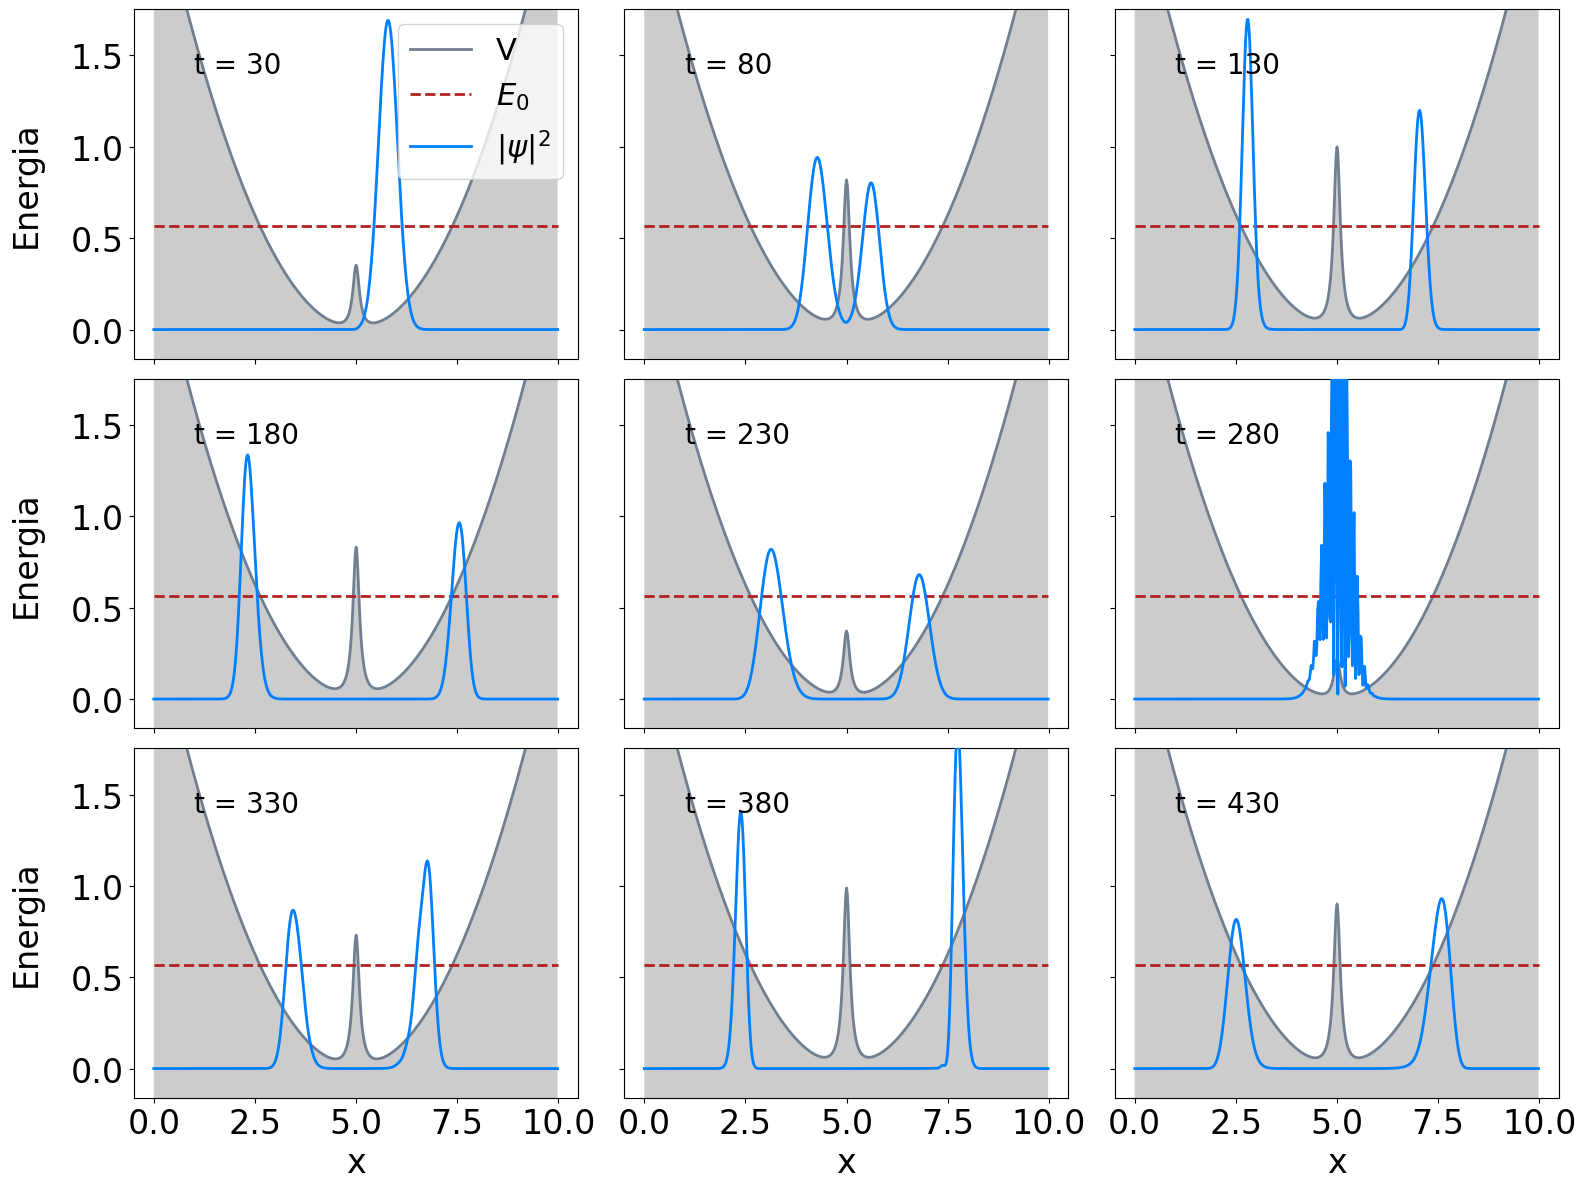
\includegraphics[width = \textwidth]{immagini/t-dep.png}
    \caption{Evoluzione di un pacchetto gaussiano di onde piano che interagisce con un potenziale dipendente dal tempo. Notare come per $t \, \approx \, 80$ la funzione d'onda venga separata tra le due regioni per poi sovrapporsi nuovamente per  $t \, \approx \, 280$ }
    \label{fig:t-dep}
\end{figure}

   
   





\chapter{Descrizione software}
\label{ch:interface}


Il software è diviso in tre componenti principali:
\begin{enumerate} [nolistsep]
    \item un ambiente grafico per la gestione dei parametri iniziali,
    \item l'algorirmo di simulazione,
    \item alcuni strumenti grafici per la visualizzazione dei risultati.
\end{enumerate}
Ognuna di queste componenti è indipendente dalle altre, poiché le informazioni sono passate attraverso file che vengono ogni volta aggiornati, in questo modo è sempre possibile risalire ai parametri utilizzati, modificarli senza usare l'ambiente grafico e gestire tutto da riga di comando.
In figura (\ref{fig:schema}) è riassunto lo schema di funzionamento. Si crea tramite l'interfaccia un file \textsl{Par.py} che riassume tutti i parametri iniziali, si lancia la simulazione dall'interfaccia, l'algoritmo simulativo salva i risultati in una cartella precedentemente selezionata. I risultati sono poi animati tramite un altro strumento grafico. Si noti che da riga di comando è possibile lanciare in maniera indipendente sia l'algoritmo simulativo sia gli strumenti di animazione, basta che siano presenti i file intermedi necessari.

Il codice è stato scritto utilizzando il linguaggio Python appoggiandosi alle librerie esterne:
\begin{itemize}[nolistsep]
    \item Numpy, per le funzioni matematiche e la gestione dei vettori,
    \item Matplotlib, per generare i grafici e le animazioni,
    \item Tkinter, per la costruzione dell'interfaccia grafica,
    \item Numba, per compilare le funzioni di evoluzione temporale.
\end{itemize}

\textcolor{red}{
Per visualizzare i risultati, oltre che al semplice strumento di animazione, sono stati implementati:
\begin{itemize}[nolistsep]
	\item uno strumento per confrontare le soluzioni numeriche con le soluzioni analitiche, 
	\item uno strumento per visualizzare l'evoluzione in contemporanea nello spazio diretto e nello spazio dei momenti,
	\item uno strumento per il calcolo dei coefficienti di riflessione e di trasmissione.
	\item uno strumento per il calcolo dei valori medi
	\item uno struemento per la valutazione dell'errore rispetto alla funzione analitica 
\end{itemize}
}

\begin{figure}
    \centering
    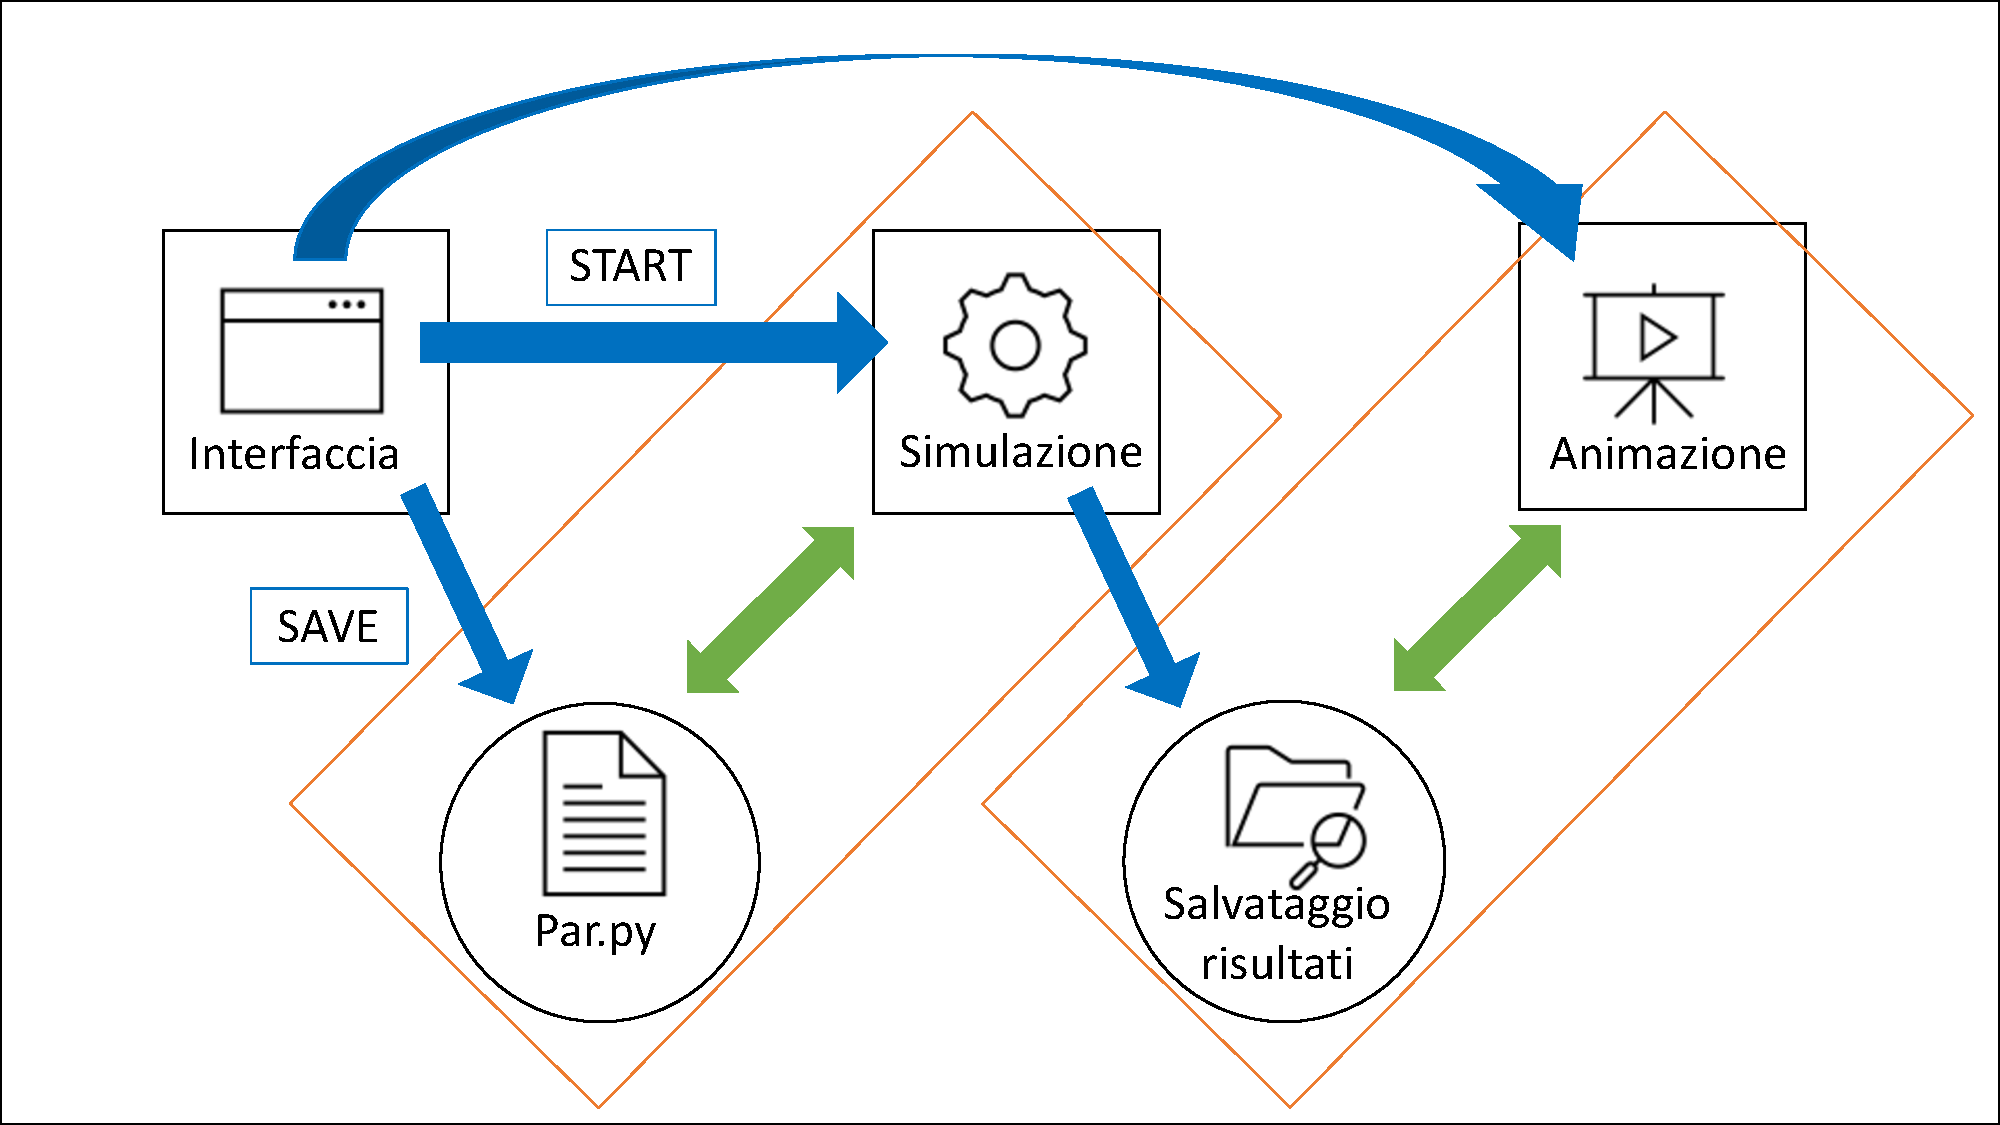
\includegraphics[width = 0.6\textwidth]{immagini/schema.pdf}
    \caption{Schema di funzionamento del software. \textcolor{red}{È una bozza se mi conferma che può andare bene la perfeziono}}
    \label{fig:schema}
\end{figure}

\begin{figure}
    \centering
    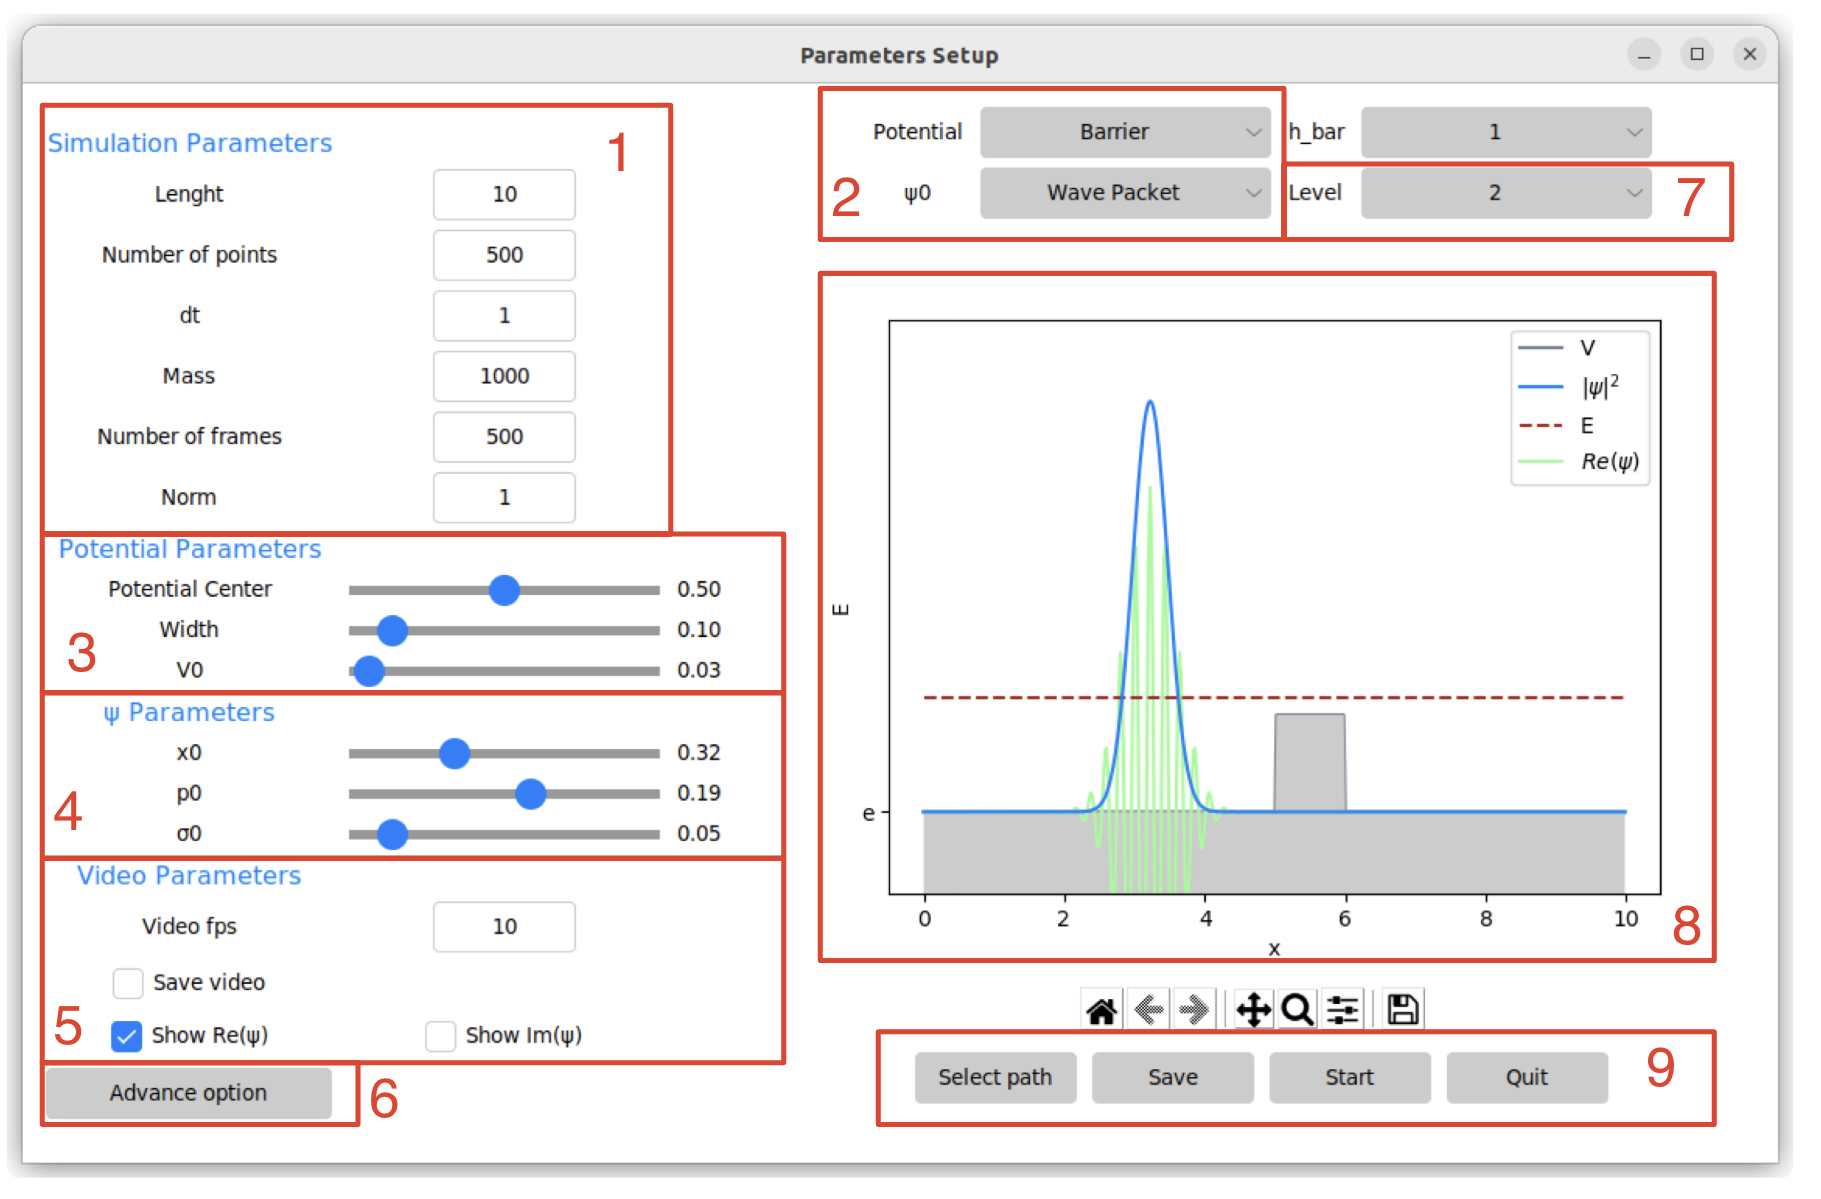
\includegraphics[width = 0.7\textwidth]{immagini/inter_num.jpg}
    \captionsetup{singlelinecheck=off}
    \caption[foo bar]{Illsustrazione dell'interfaccia.
    \small{
    \begin{enumerate}[nolistsep]
        \item Si possono modificare i parametri caratteristici dello spazio e della particella, nonché impostare il numero e la grandezza dei passi temporali da eseguire.
        \item Permette di scegliere tra gli stati e i potenziali citati al capitolo (\ref{ch:applicazioni}).
        \item È possibile modificare i parametri caratteristici del potenziale selezionato.
        \item È possibile modificare i parametri caratteristici dello stato iniziale selezionato. Quando si modificano parametri che influenzano la funzione d'onda nello spazio dei momenti viene messa in mostra un'anteprima dello stato iniziale nello spazio dei momenti. 
        \item  Si possono modificare alcuni parametri per la creazione dell'animazione finale. Tra questi è possibile mostrare la parte reale e immaginaria della soluzione.
        \item Tra le opzioni avanzate si può selezionare l'algoritmo di simulazione, vedi sezione (\ref{sec:ev_code}), e inserire dei controlli per la conservazione della norma e dell'energia.
        \item Il parametro  \textsl{Level} indica l'ordine a cui viene troncata l'espansione in eq. (\ref{eq:LT_expantion}).
        \item Viene visualizzata in diretta un'anteprima dello stato iniziale.
        \item Cliccando sui seguenti tasti si controllano le funzioni dell'interfaccia. Per eseguire in maniera corretta la simulazione la procedura prevista è: selezionare il percorso di salvataggio, salvare i risultati, far partire la simulazione e attendere l'animazione, uscire.    
    \end{enumerate}
    } }
    \label{fig:interface}
\end{figure}

\section{Algoritmo di simulazione}
\label{sec:ev_code}

Il cuore dell'algoritmo di simulazione è un ciclo che richiama ad ogni iterazione una funzione di evoluzione e salva i risultati nella cartella indicata dall'utente.
Sono state implementate tre diverse funzioni di evoluzione che differiscono per generalità e prestazioni. Inoltre l'utente può scegliere tra due tipologie di algoritmi di simulazione: con o senza anteprima, dove con anteprima si intende una visualizzazioni in diretta dei risultati della simulazione. Questa scelta è dovuta alla perdita di velocità causata dalla creazione immediata dei grafici.
Di seguito si riporta il codice utilizzato per la più generica funzione di evoluzione, con la quale è possibile simulare un potenziale dipendente dal tempo e selezionare l'ordine a cui viene troncata l'espansione.
\begin{lstlisting}[language = Python]
@jit
def evolution_t_dependent(y, q, k, dt, V, m, mat_f, mat_i, 
            N, L, h, P_MAX, f_zero, coefficients, Level):
    for i in range(Level):
        if coefficients[i][0] != 0:
            # V terms application
            y = exp_V(y, V, dt, h, coefficients[i][0])
        if coefficients[i][1] != 0:
            # Fourier transform 
            f_y = DFT.Dft(y ,q, k, mat_f, N, L, h, f_zero)   

            f_y = DFT.shift(f_y, k, P_MAX)
            k = DFT.shift_p(k, P_MAX)

            # T terms application
            f_y = exp_T(f_y, k, m, dt, h, coefficients[i][1])      

            f_y = DFT.back_shift(f_y, k)
            k = DFT.back_shift_p(k, P_MAX)

            # Anti-Fourier transform
            y= DFT.iDft(f_y, q, k, mat_i, L, h, f_zero)   
    return y
\end{lstlisting}
Il simbolo \textsl{@jit} è detto \textsl{decorator} e serve per compilare la funzione attraverso Numba. Tale processo rende il calcolo molto più rapido, ma per poter sfruttare al meglio le potenzialità di questo compilatore bisogna rinunciare ad alcune comodità tipiche dei linguaggi interpretati come Python. Numba richiede, infatti, che tutte le variabili utilizzate nella funzione siano passate come parametri e che le variabili siano di tipo statico. Per questo vengono inseriti tra i parametri alcuni termini che non hanno a che fare con l'evoluzione del sistema, ma che sono utilizzati come variabili di appoggio, come ad esempio \textsl{f\_zero}.
DFT è la libreria personale utilizzata per raggruppare i metodi che computano la trasformata di Fourier. Si ricorda che per poter applicare i termini a cui esponente compare $\hat{T}$ oltre che applicare la trasformata di Fourier è anche necessario traslare la soluzione, questo viene fatto tramite i metodi \textsl{shift}, vedi sezione (\ref{sec:DFT}). Per rendere il codice più efficiente, le matrici, \textsl{mat\_f} e \textsl{mat\_i}, utilizzate per calcolare le trasformate sono precalcolate e vengono passate alle funzioni come parametri.
Il parametro \textsl{coefficients} rappresenta un vettore di dimensioni $Level \times 2$ che raggruppa i coefficienti $c_j$ e $d_j$ dell'espansione. 
Le funzioni \textsl{exp\_V} e \textsl{exp\_T} restituiscono semplicemente i termini esponenziali che compaiono nell'espansione. La funzione può essere resa più efficiente in quei casi in cui è possibile precalcolare alcuni termini. Per i potenziali non dipendenti dal tempo, infatti, i risultati resistituiti dalle funzioni \textsl{exp\_V} e \textsl{exp\_T} sono sempre gli stessi. Quindi risulta più efficiente precalcolari e passarli come parametri, in modo da dover eseguire solo una moltiplicazione. Con questa modifica si ottiene la seconda versione della funzione di evoluzione.
Rinunciando ad un ulteriore grado di libertà si può rendere la funzione ancora più efficiente. Infatti e prestazioni del compilatore Numba sono infatti piuttosto sensibili alla presenza di condizioni \textsl{if} e di condizioni sui cicli. Se si elimina il ciclo \textsl{for} per sostituirlo con una serie operazioni da eseguire tutte in fila e si eliminano manualmente i termini nulli si ottiene un considerevole aumento nelle prestazioni. Per poter implemenatare una tale funzione è quindi necessario conoscere in precedenza sia il livello sia i coefficienti associati a tale livello. Nel codice è stato implementata una funzione di quest'ultimo tipo per il livello che corrisponde a troncare l'espansione a $O(\delta t^{\, 3})$.







\clearpage

\addcontentsline{toc}{chapter}{Conclusioni} % Capitolo non numerato
\chapter*{Conclusioni}
\label{ch:conclusioni}

Grazie al lavoro esposto in sezione (\ref{ch:Validazione}) è possibile affermare che la soluzione numerica
%cambia
generata tramite la simulazione è  del tutto compatibile con la soluzione esatta. 
È quindi possibile utilizzare questo strumento per risolvere un qualsiasi problema monodimensionale e ottenere risultati concreti come in sezione (\ref{ch:applicazioni}). 

%amplia
Il formalismo esposto in sezione (\ref{ch:teoria}) è dunque verificatto e applicato. Tale formalismo è generalizzabile per qualsiasi operatore $\hat{H}$ in un numero arbitario di dimensioni, quindi si può estendere ad ogni sistema quantistico. I problemi che si possono riscontrare nella generalizzazione, oltre al fatto che la comprensione delle formule matematica diviene più difficoltosa, riguardano soprattutto il costo computazionale e le strategie di visualizzazione dei risultati. Ogni volta che si aumentano le dimensioni o i gradi di libertà del sistema (ad esempio considerando lo spin), è necessario ampliare la grandezza dei vettori che contengono la funzione d'onda. Nello spazio delle coordinate l'aumento di punti da considerare scala con $N^d$, dove di rappresenta le dimensioni. Inoltre per rappresentare funzioni d'onda multidimensionali è necessario animare uno spazio tridimesionale o quadridimensionale, il che anche se possibile rende i risultati più difficili da interpretare. 


\chapter*{Ringraziamenti}

\printbibliography
\nocite{*}

\end{document}
